% ============================================================
% CHAPITRE 4 : MODELISATION - CONCEPTION DU MOTEUR AGENTIQUE
% CRISP-DM - PHASE 4 (Modeling)
% Structure canonique :
%   4.1 Selection des techniques de modelisation
%   4.2 Conception du protocole de test
%   4.3 Construction des modeles
%   4.4 Evaluation interne des modeles
%
% Figures : docs/rapport/img/fig_*.png  (generees par figures.py)
% Bibliographie : docs/rapport/references.bib
% ============================================================

\chapter{Modélisation : conception du moteur agentique}
\label{chap:modelisation}

% ------------------------------------------------------------
\section*{Introduction}
\addcontentsline{toc}{section}{Introduction}
% ------------------------------------------------------------

Le chapitre précédent a produit un jeu de données vérifié, préparé et documenté, et a fixé le protocole de découpage temporel sous lequel toute performance devra être obtenue. Le présent chapitre conduit la quatrième phase de CRISP-DM : la modélisation. Il décrit les modèles retenus, les justifie au regard des objectifs analytiques et des propriétés des données observées, et présente l'architecture logicielle qui les met en œuvre.

L'ordre suivi n'est pas neutre. Il aurait été possible de présenter l'architecture au chapitre~\ref{chap:comprehension-metier}, comme le font de nombreux rapports d'ingénierie, en la traitant comme un préalable technique. Ce choix a été écarté : CRISP-DM veut le problème posé et les données comprises \textit{avant} la technique, précisément pour éviter que l'architecture ne détermine les objectifs plutôt que l'inverse. L'architecture présentée ici est donc une conséquence des objectifs du chapitre~\ref{chap:comprehension-metier} et des constats du chapitre~\ref{chap:donnees}, et chaque décision de conception majeure est rattachée à celui des deux qui la motive.

Un principe traverse l'ensemble du chapitre et mérite d'être énoncé d'emblée, car il commande la quasi-totalité des choix qui suivent : \textbf{les calculs qui engagent une décision restent déterministes ; le modèle de langage formule, il ne calcule pas}. Une quantité de commande, un point de réapprovisionnement, un score de risque, un écart à l'objectif sont produits par des fonctions de calcul vérifiables et reproductibles. Le modèle de langage intervient en aval, pour expliquer, hiérarchiser et formuler, jamais pour produire le nombre qui engage. Ce principe n'est pas une précaution de style : il est la condition pour qu'une recommandation soit auditable, et donc pour qu'un responsable puisse en assumer la validation.

Le chapitre s'ouvre sur l'architecture générale de la solution (section~\ref{sec:architecture}), puis présente la sélection des techniques de modélisation (section~\ref{sec:selection-techniques}) et la conception du protocole de test (section~\ref{sec:protocole-test}). Viennent ensuite les modèles proprement dits : prévision du chiffre d'affaires et détection d'anomalies (section~\ref{sec:modele-ca}), prévision de la demande par référence (section~\ref{sec:modele-demande}), modèles de décision de stock (section~\ref{sec:decision-stock}). La conception des agents intelligents et de la base de connaissances occupe les sections~\ref{sec:agents} et~\ref{sec:rag}. L'orchestration multi-agents, le contrôle de conformité et la robustesse de la chaîne de génération closent le chapitre (sections~\ref{sec:orchestration} à~\ref{sec:robustesse}).

% ------------------------------------------------------------
\section{Architecture générale de la solution}
\label{sec:architecture}
% ------------------------------------------------------------

\subsection{Architecture en trois tiers}

La solution adopte une architecture en trois tiers, dont la figure~\ref{fig:archi-trois-tiers-chap4} donne la vue d'ensemble.

\begin{figure}[H]
    \centering
    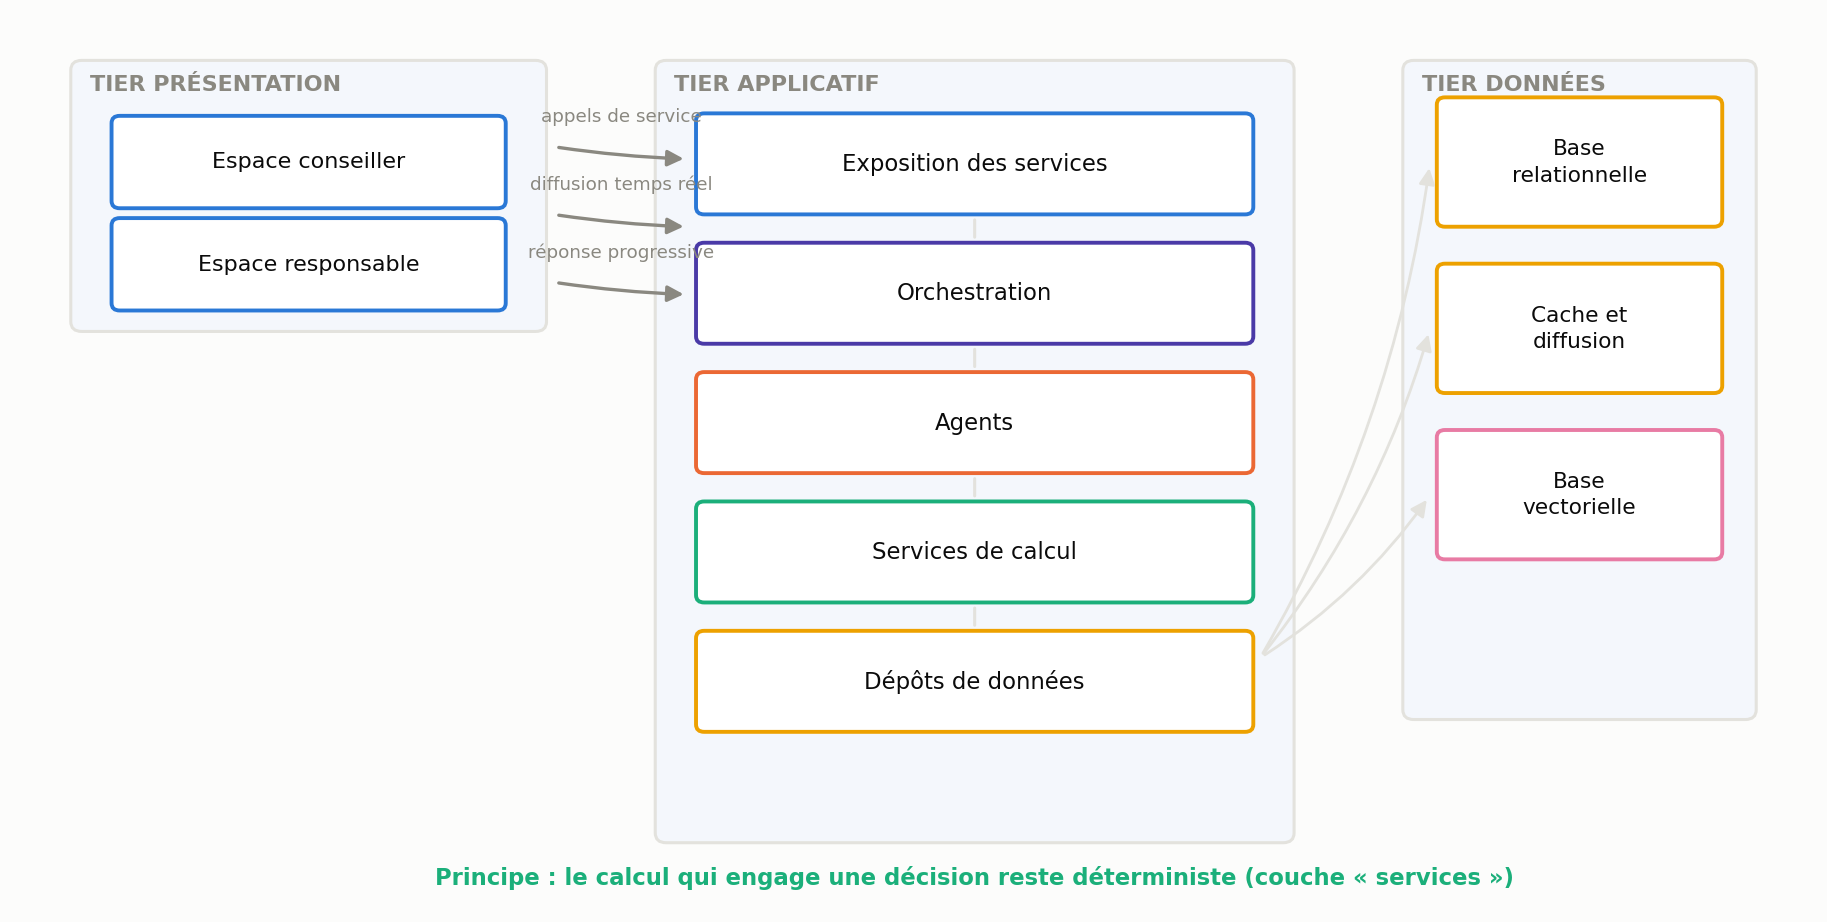
\includegraphics[width=\textwidth]{img/fig_archi_trois_tiers.png}
    \caption{Architecture générale en trois tiers}
    \label{fig:archi-trois-tiers-chap4}
\end{figure}

Le \textbf{tier de présentation} est une application web à page unique, destinée aux deux profils d'utilisateurs identifiés au chapitre~\ref{chap:comprehension-metier} : le conseiller de vente et le responsable de point de vente. Il communique avec le tier applicatif par trois canaux de nature différente : des appels de service classiques pour les consultations, un canal de diffusion permanent pour les mises à jour temps réel, et un canal de réponse progressive pour l'assistant conversationnel. Le choix de trois canaux plutôt qu'un seul répond à des besoins distincts : une consultation de tableau de bord tolère une latence de quelques centaines de millisecondes, une alerte de rupture doit parvenir sans sollicitation du client, et une réponse conversationnelle doit s'afficher au fil de sa génération sous peine de paraître figée.

Le \textbf{tier applicatif} héberge l'ensemble de la logique : exposition des services, orchestration des agents, agents eux-mêmes, services de calcul et dépôts d'accès aux données. Il est organisé en couches strictes décrites ci-dessous.

Le \textbf{tier de données} rassemble la base relationnelle décrite au chapitre~\ref{chap:donnees}, un cache en mémoire assurant à la fois la mise en cache des calculs coûteux et la diffusion d'événements entre composants, et une base vectorielle supportant la recherche documentaire.

\subsection{Architecture logique en couches}

La figure~\ref{fig:archi-couches-chap4} détaille l'organisation interne du tier applicatif.

\begin{figure}[H]
    \centering
    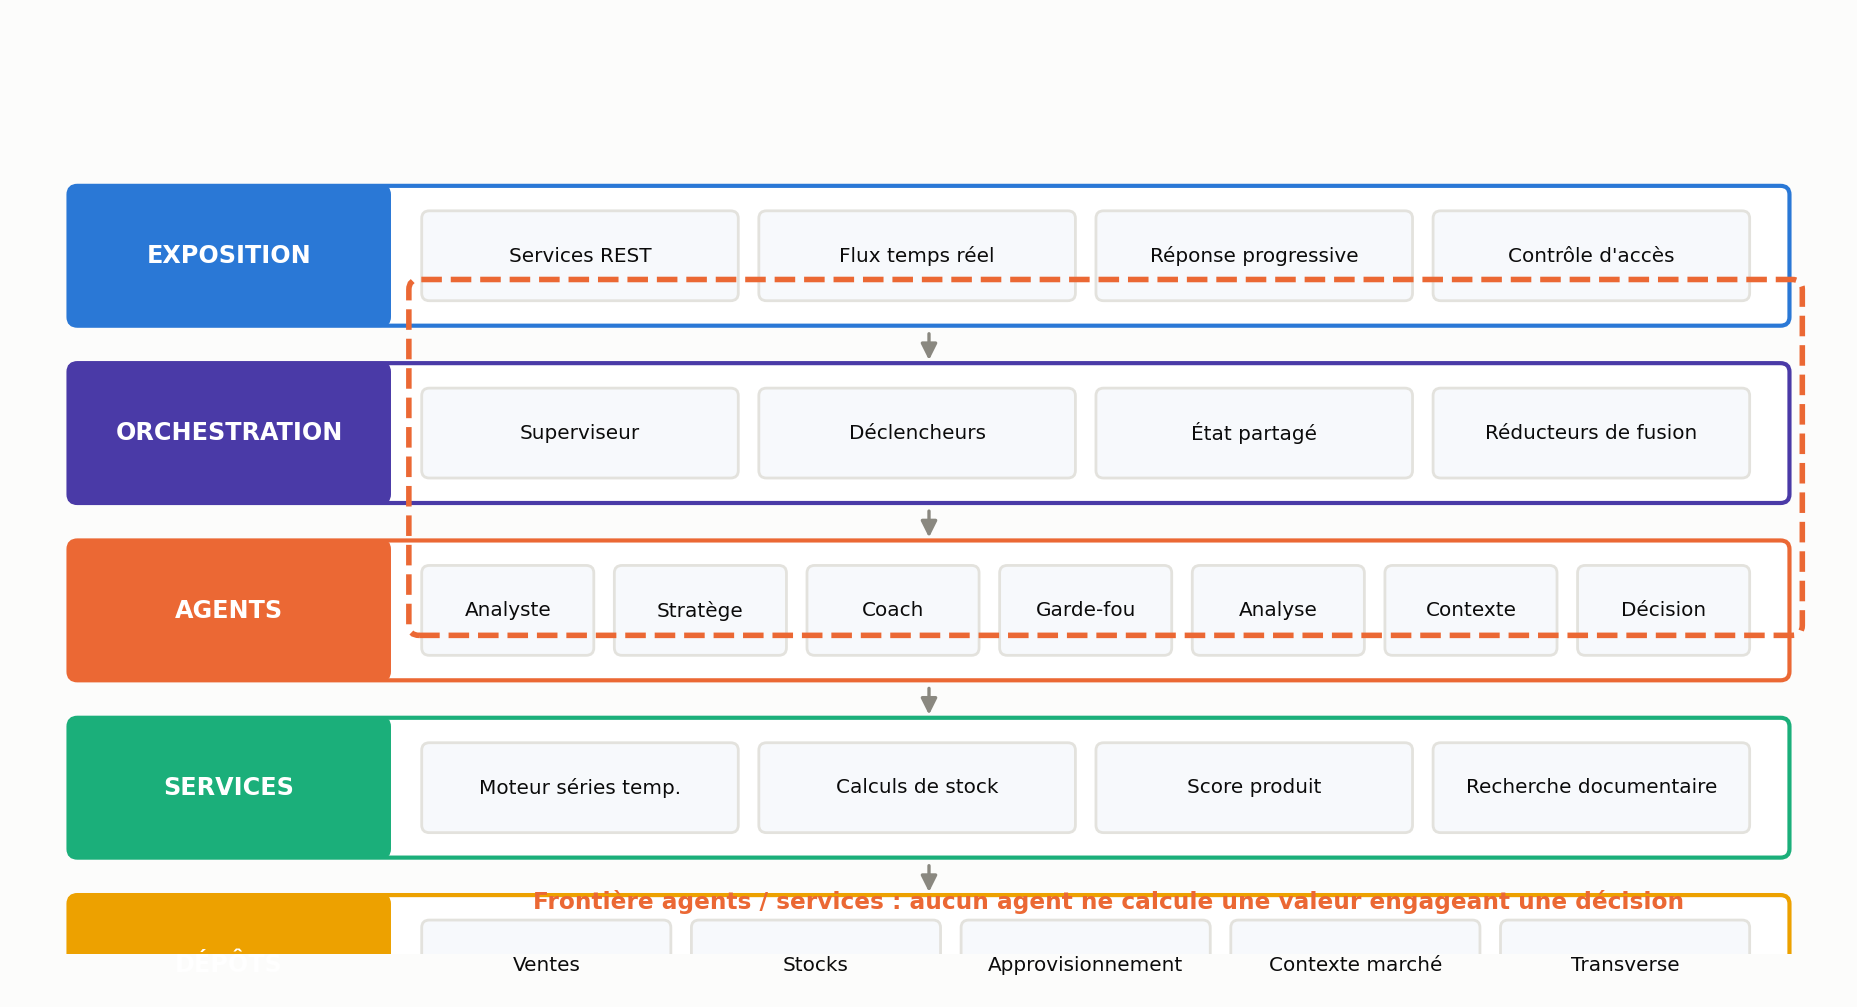
\includegraphics[width=\textwidth]{img/fig_archi_couches.png}
    \caption{Architecture logique en couches du tier applicatif}
    \label{fig:archi-couches-chap4}
\end{figure}

Cinq couches se succèdent, chacune ne dépendant que de la suivante. La couche d'\textbf{exposition} traduit les requêtes entrantes en appels applicatifs et applique le contrôle d'accès. La couche d'\textbf{orchestration} détermine quels agents mobiliser, dans quel ordre, et fusionne leurs productions. La couche des \textbf{agents} contient les unités de raisonnement proprement dites. La couche des \textbf{services} regroupe les calculs métier déterministes : moteur de séries temporelles, calculs de stock, scoring produit. La couche des \textbf{dépôts} isole l'accès aux données.

La frontière entre couche des agents et couche des services est la matérialisation logicielle du principe énoncé en introduction. Les agents n'exécutent aucun calcul décisif : ils appellent des services qui le font. Cette séparation a une conséquence pratique décisive pour l'évaluation : les calculs sont testables unitairement, indépendamment de tout modèle de langage, ce qui permet une couverture de tests que le caractère non déterministe des modèles génératifs rendrait autrement impossible.

\subsection{Répartition des responsabilités entre calcul et formulation}

Le tableau~\ref{tab:repartition-chap4} explicite cette répartition, objectif analytique par objectif analytique.

\begingroup
\setlength{\tabcolsep}{3pt}
\renewcommand{\arraystretch}{1.15}
\small

\begin{longtable}{|P{1.2cm}|P{5.9cm}|P{5.9cm}|}
\hline
\rowcolor{red!75}
\textcolor{white}{\textbf{Réf.}} &
\textcolor{white}{\textbf{Calculé de façon déterministe}} &
\textcolor{white}{\textbf{Confié au modèle de langage}} \\
\hline
\endhead
\hline
\endfoot
\hline
\endlastfoot
OD-1 & Prévision de fin de journée, intervalle, tendance & Rien \\
\hline
OD-2 & Écart horaire, score normalisé, statut & Formulation du diagnostic \\
\hline
OD-3 & Demande prévue de référence, correction contextuelle & Rien \\
\hline
OD-4 & Couverture, classe de risque & Arbitrage des conflits entre dimensions \\
\hline
OD-5 & Stock de sécurité, point de commande, quantité économique, arrondi aux contraintes & Justification de la décision, choix de l'action parmi celles autorisées \\
\hline
OD-6 & Score multicritère et rang des produits & Message de recommandation adressé au conseiller \\
\hline
OD-7 & Recherche, fusion des classements, seuils de pertinence & Synthèse ancrée sur les extraits retrouvés \\
\hline
OD-8 & Application des règles de conformité, verdict & Rien \\
\hline
\caption{Répartition des responsabilités entre calcul déterministe et formulation générative}
\label{tab:repartition-chap4}
\end{longtable}
\endgroup

Trois lignes de ce tableau portent la mention « rien » dans la colonne générative. Ce n'est pas un oubli mais une décision : pour la prévision de chiffre d'affaires, la prévision de demande et le verdict de conformité, aucune intervention d'un modèle de langage n'est admise, y compris à titre de reformulation, car toute reformulation d'un nombre porte le risque de l'altérer.

\subsection{Diagramme de composants}

La figure~\ref{fig:composants-chap4} présente les composants applicatifs et leurs dépendances.

\begin{figure}[H]
    \centering
    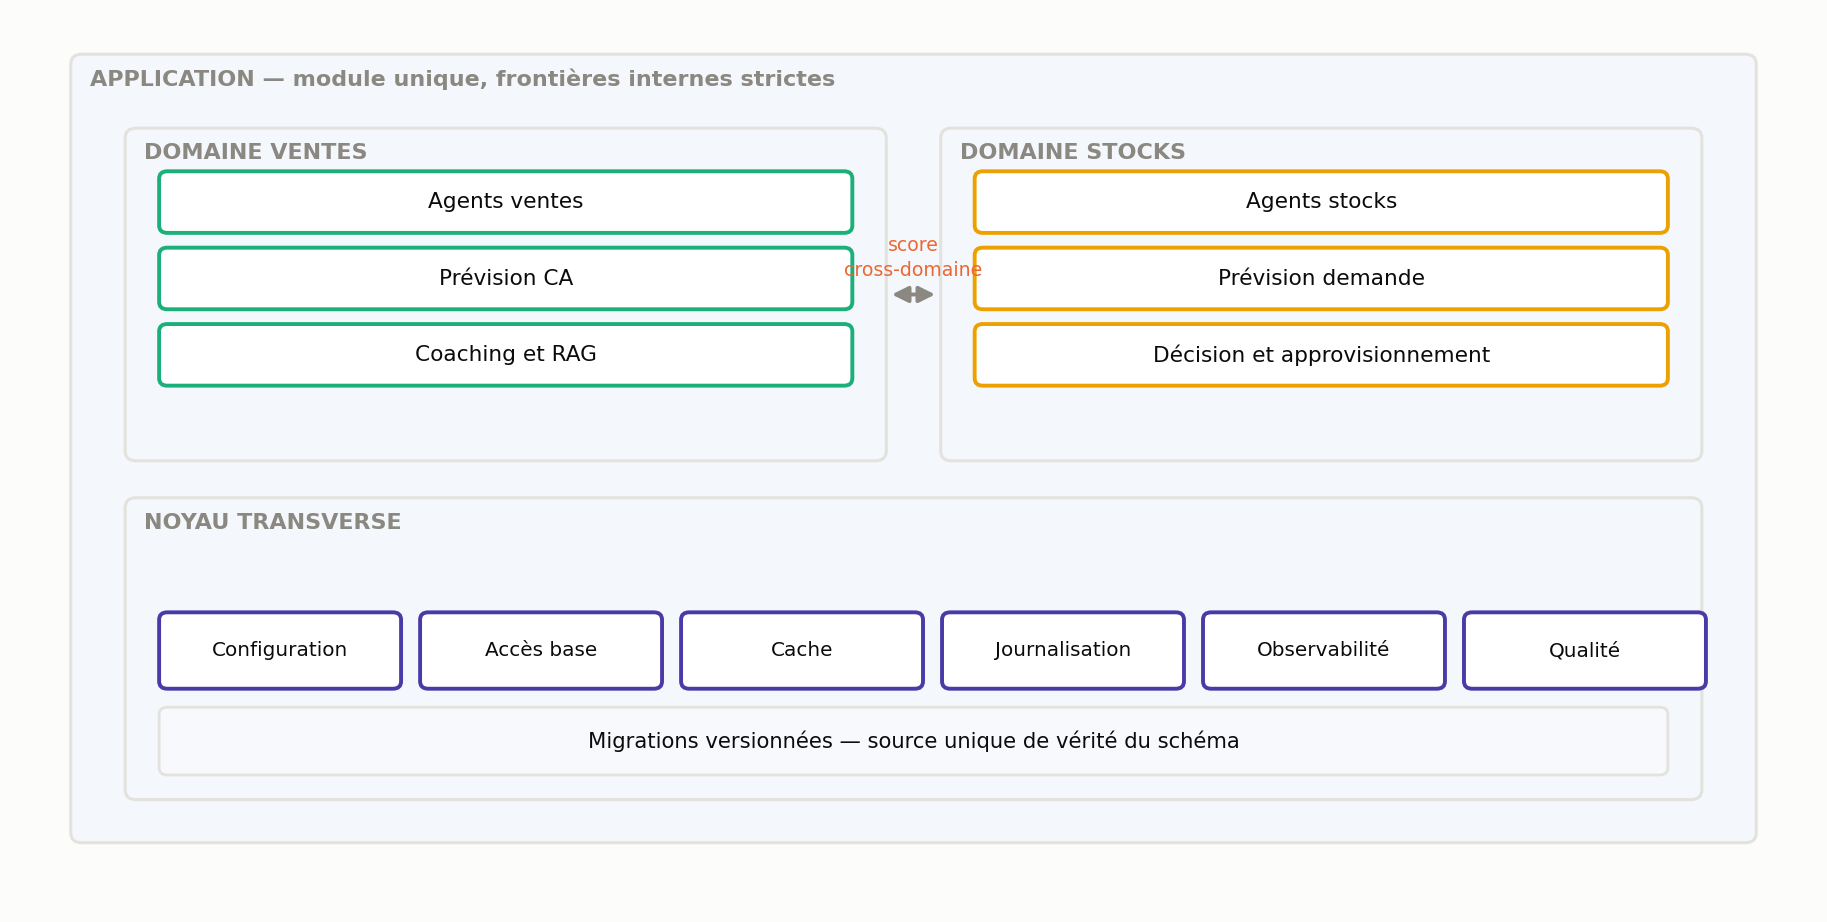
\includegraphics[width=\textwidth]{img/fig_composants.png}
    \caption{Diagramme de composants de la solution}
    \label{fig:composants-chap4}
\end{figure}

L'application est organisée en un module unique regroupant deux domaines métier -- ventes et stocks -- et un noyau transverse. Cette organisation monolithique modulaire a été retenue au terme d'une refonte : le projet a d'abord été structuré en modules déployés séparément, ce qui multipliait les configurations, les connexions à la base et les points de défaillance sans bénéfice réel à l'échelle considérée. Le regroupement en un module unique, avec des frontières internes strictes entre domaines, conserve la séparation conceptuelle sans en payer le coût opérationnel.

\subsection{Diagramme de classes des entités métier}

La figure~\ref{fig:classes-chap4} présente les entités métier manipulées par les agents et les services.

\begin{figure}[H]
    \centering
    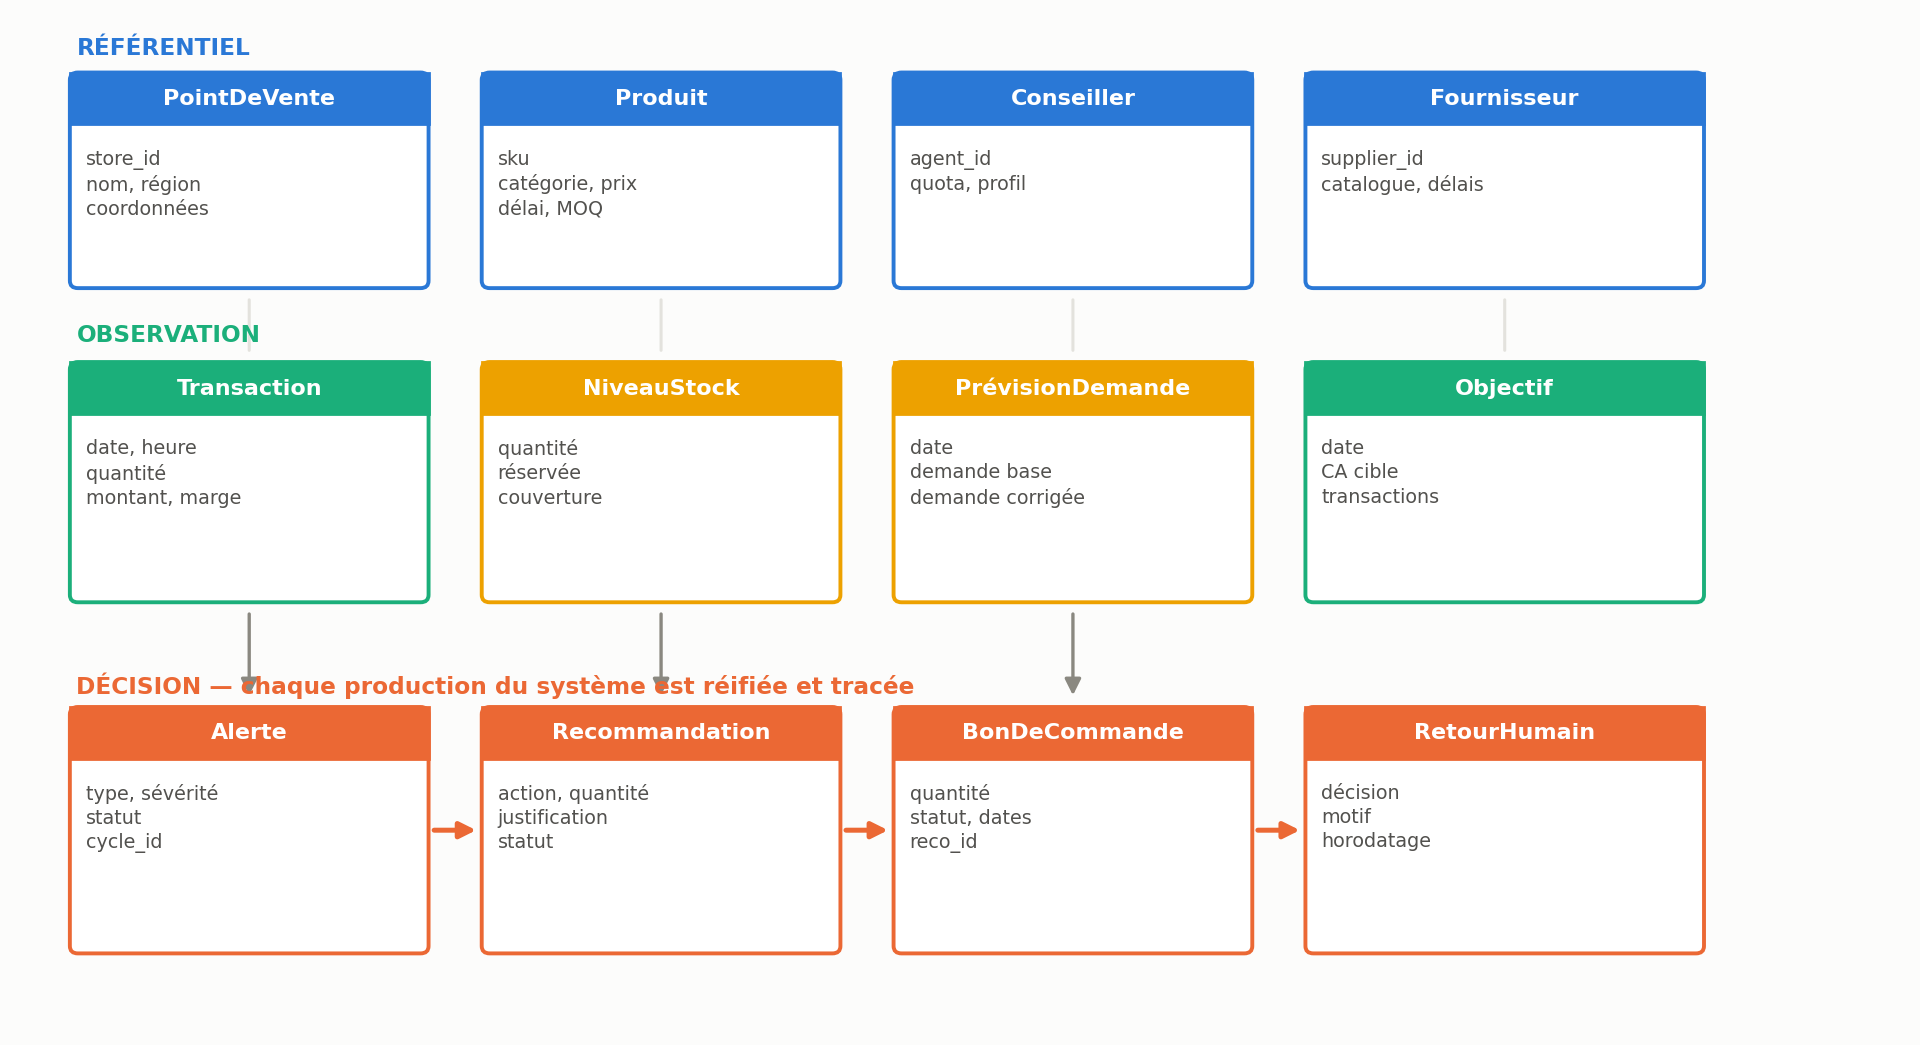
\includegraphics[width=\textwidth]{img/fig_classes_metier.png}
    \caption{Diagramme de classes des entités métier}
    \label{fig:classes-chap4}
\end{figure}

Les entités se répartissent en trois familles. Les entités de \textbf{référentiel} -- point de vente, produit, conseiller, fournisseur -- sont stables et partagées. Les entités d'\textbf{observation} -- transaction, niveau de stock, objectif -- portent les faits mesurés. Les entités de \textbf{décision} -- alerte, recommandation, bon de commande, validation humaine, retour de feedback -- portent les productions du système. Cette dernière famille est la plus significative sur le plan de la conception : chaque production du système est réifiée en objet persistant, doté d'un identifiant, d'un état et d'une trace de son origine. Un système dont les recommandations ne seraient que des chaînes de caractères transmises à l'interface ne pourrait ni être évalué a posteriori, ni supporter la boucle de retour humain exigée par l'objectif OD-8.

% ------------------------------------------------------------
\section{Sélection des techniques de modélisation}
\label{sec:selection-techniques}
% ------------------------------------------------------------

La première tâche de la phase de modélisation consiste à choisir, pour chaque objectif analytique, la ou les techniques candidates, et à vérifier que leurs hypothèses sont satisfaites par les données du chapitre~\ref{chap:donnees}. Le tableau~\ref{tab:techniques-chap4} présente cette sélection.

\begingroup
\setlength{\tabcolsep}{3pt}
\renewcommand{\arraystretch}{1.15}
\small

\begin{longtable}{|P{1.1cm}|P{3.6cm}|P{4.4cm}|P{4.0cm}|}
\hline
\rowcolor{red!75}
\textcolor{white}{\textbf{Réf.}} &
\textcolor{white}{\textbf{Techniques candidates}} &
\textcolor{white}{\textbf{Hypothèse et vérification}} &
\textcolor{white}{\textbf{Décision}} \\
\hline
\endhead
\hline
\endfoot
\hline
\endlastfoot
OD-1 & Référence naïve saisonnière ; moyennes mobiles ; lissage exponentiel saisonnier ; modèle appris global à gradient boosté & Saisonnalité hebdomadaire marquée : \textbf{vérifiée} (fig.~\ref{fig:saisonnalite-hebdo-chap3}). Historique annuel suffisant : \textbf{non vérifié} & Les quatre familles sont retenues en concurrence et départagées au chapitre~\ref{chap:evaluation}. Composante annuelle écartée \\
\hline
OD-2 & Seuil fixe sur l'objectif ; écart au profil horaire attendu avec score normalisé & Profil horaire stable et non uniforme : \textbf{vérifiée} (fig.~\ref{fig:profil-horaire-chap3}) & Écart au profil retenu ; seuil fixe écarté (saturation d'alertes en début de journée) \\
\hline
OD-3 & Décomposition saisonnière multiple ; modèle appris sur variables exogènes ; combinaison des deux en cascade & Historique par référence suffisant : \textbf{vérifiée seulement au-delà du seuil d'inclusion} (fig.~\ref{fig:pareto-chap3}) & Cascade retenue : base statistique corrigée par modèle appris. Repli par règle de seuil hors périmètre \\
\hline
OD-4 & Seuils de gestion ; calcul par la couverture et le délai ; combinaison des deux & Bimodalité de la couverture : \textbf{vérifiée} (fig.~\ref{fig:couverture-chap3}) & Classification à deux couches, la plus sévère l'emportant \\
\hline
OD-5 & Formulation classique de la gestion de stock : stock de sécurité, point de commande, quantité économique & Demande approximativement normale sur l'horizon du délai : \textbf{admise}, écart documenté & Formulation classique retenue, avec niveau de service ajusté au cycle de vie \\
\hline
OD-6 & Tri par marge ; tri par disponibilité ; score multicritère pondéré & Décorrélation entre disponibilité et potentiel : \textbf{vérifiée} (fig.~\ref{fig:correlation-chap4}) & Score multicritère retenu ; tris simples écartés comme non informatifs \\
\hline
OD-7 & Recherche lexicale seule ; recherche sémantique seule ; recherche hybride avec fusion des classements & Corpus multilingue et à vocabulaire spécialisé : \textbf{vérifiée} & Recherche hybride retenue \\
\hline
OD-8 & Règles déterministes ; classification par modèle de langage ; combinaison & Exigence d'auditabilité du verdict : \textbf{contrainte métier} & Règles déterministes seules pour le verdict ; évaluation générative réservée au suivi a posteriori \\
\hline
\caption{Sélection des techniques de modélisation par objectif analytique}
\label{tab:techniques-chap4}
\end{longtable}
\endgroup

Trois rejets méritent d'être motivés, car une sélection sans rejet documenté n'est pas une sélection.

Le \textbf{seuil fixe} pour la détection d'anomalies horaires a été écarté sur la seule foi de la figure~\ref{fig:profil-horaire-chap3} : la forme du profil garantit qu'un tel seuil produirait des alertes massives en début de journée et un silence en fin de journée. Aucun réglage de seuil ne corrige un défaut de forme.

La \textbf{composante saisonnière annuelle} a été écartée faute d'historique : vingt-deux mois n'autorisent pas l'estimation d'un cycle annuel avec une confiance suffisante. Les effets calendaires annuels sont donc représentés par des variables exogènes explicites -- Ramadan, rentrée, fêtes -- plutôt que par une décomposition, ce qui présente l'avantage supplémentaire de rester interprétable.

La \textbf{classification du verdict de conformité par modèle de langage} a été écartée pour une raison de nature : un verdict qui bloque la diffusion d'une recommandation doit pouvoir être expliqué par la règle qui l'a produit et rejoué à l'identique. Un modèle génératif ne garantit ni l'un ni l'autre. L'évaluation générative n'est pas abandonnée pour autant : elle est employée en supervision a posteriori, où sa variabilité est acceptable et sa richesse d'analyse précieuse.

% ------------------------------------------------------------
\section{Conception du protocole de test}
\label{sec:protocole-test}
% ------------------------------------------------------------

CRISP-DM place la conception du protocole de test dans la phase de modélisation, avant la construction des modèles. Cette antériorité est une garantie méthodologique : un protocole conçu après l'obtention des résultats risque toujours d'avoir été choisi parce qu'il les flatte.

Pour les objectifs quantitatifs OD-1 et OD-3, la métrique principale retenue est l'\textbf{erreur absolue pondérée}, définie comme le rapport entre la somme des erreurs absolues et la somme des valeurs réelles :

\begin{equation}
\mathrm{WAPE} = \frac{\sum_{t} \left| y_t - \hat{y}_t \right|}{\sum_{t} \left| y_t \right|}
\end{equation}

Ce choix, conforme aux recommandations de la littérature de prévision \cite{hyndman2021fpp,makridakis2020m4}, se justifie par deux propriétés. D'une part, cette métrique reste définie lorsque des valeurs réelles sont nulles, situation fréquente sur la demande par référence, là où une erreur relative moyenne diverge. D'autre part, elle pondère naturellement les erreurs par le volume, ce qui est le comportement souhaité en gestion : se tromper de dix unités sur une référence qui en vend mille est sans conséquence, se tromper de dix unités sur une référence qui en vend douze en a.

Une métrique complémentaire est retenue pour situer la performance par rapport à une référence naïve :

\begin{equation}
\mathrm{MASE} = \frac{\frac{1}{n}\sum_{t} \left| y_t - \hat{y}_t \right|}{\frac{1}{n-m}\sum_{t>m} \left| y_t - y_{t-m} \right|}
\end{equation}

où $m$ désigne la période saisonnière. Une valeur inférieure à un signifie que le modèle bat la référence naïve saisonnière ; une valeur supérieure signifie qu'il lui est inférieur, quel que soit son degré de sophistication. Cette métrique est l'unique garde-fou contre le biais le plus courant en modélisation : conclure qu'un modèle est bon parce que son erreur paraît faible, sans jamais vérifier qu'une méthode triviale ne ferait pas mieux.

Le biais moyen est également suivi, afin de détecter une surestimation ou une sous-estimation systématique, invisible dans les métriques d'erreur absolue mais lourde de conséquences en gestion de stock où elle se traduit par un surstock ou une rupture structurels.

Pour les objectifs textuels OD-6 à OD-8, aucune métrique d'erreur ne s'applique. Le protocole retenu combine trois niveaux : des \textbf{contrôles déterministes} vérifiant des propriétés objectivement décidables -- absence de remise non autorisée, absence de produit indisponible, langue de la réponse, absence de fuite d'instructions ; une \textbf{évaluation par juge automatique} \cite{zheng2023judge} notant sur une grille fermée des critères qualitatifs ; et le \textbf{retour humain} du responsable, seul juge de la pertinence métier réelle. Les limites de l'évaluation par juge automatique sont discutées au chapitre~\ref{chap:evaluation}, où elles sont explicitement assumées.

% ------------------------------------------------------------
\section{Modélisation prédictive du domaine Ventes}
\label{sec:modele-ca}
% ------------------------------------------------------------

\subsection{Moteur de séries temporelles}

Le cœur du domaine Ventes est un moteur de séries temporelles entièrement déterministe, qui n'invoque aucun modèle de langage et produit sa sortie en moins d'une seconde. Cette contrainte de latence n'est pas gratuite : elle découle de l'exigence BNF-1 du chapitre~\ref{chap:comprehension-metier}, elle-même issue du contexte d'usage -- un conseiller au comptoir, entre deux clients.

Le moteur enchaîne six traitements sur la série de chiffre d'affaires journalier du point de vente.

Le premier est un \textbf{lissage exponentiel saisonnier} de période hebdomadaire, dans sa formulation additive \cite{holt2004forecasting,winters1960forecasting}. Le modèle décompose la série en un niveau $\ell_t$, une tendance $b_t$ et une composante saisonnière $s_t$ :

\begin{align}
\ell_t &= \alpha \left( y_t - s_{t-m} \right) + (1-\alpha)\left( \ell_{t-1} + b_{t-1} \right) \\
b_t &= \beta \left( \ell_t - \ell_{t-1} \right) + (1-\beta)\, b_{t-1} \\
s_t &= \gamma \left( y_t - \ell_t \right) + (1-\gamma)\, s_{t-m}
\end{align}

avec $m = 7$. La prévision à l'horizon $h$ s'écrit $\hat{y}_{t+h} = \ell_t + h\,b_t + s_{t+h-m}$. Les paramètres de lissage sont déterminés par recherche sur grille, l'objectif d'optimisation étant l'erreur mesurée en rétro-test à origine glissante et non l'erreur d'ajustement sur l'historique -- distinction essentielle, la seconde récompensant le surajustement.

Le deuxième traitement est l'estimation du \textbf{profil intra-journalier} par jour de semaine, c'est-à-dire la part du chiffre d'affaires journalier réalisée à chaque heure. Sept profils sont estimés, conformément au constat du chapitre~\ref{chap:donnees}.

Le troisième est la \textbf{prévision hybride de fin de journée}. En début de journée, la prévision repose entièrement sur le modèle de série temporelle. À mesure que la journée avance, le réalisé cumulé prend le pas : la prévision devient une combinaison du modèle et de l'extrapolation du réalisé par le profil horaire, avec un poids qui croît avec l'avancement de la journée. Cette construction est ce qui permet à la prévision d'être \textit{utile} : une prévision de fin de journée qui ne tiendrait pas compte de ce qui s'est déjà vendu à quinze heures n'aurait aucune valeur d'aide à la décision.

Le quatrième est le \textbf{calcul de l'écart horaire}, qui répond directement à l'objectif OD-2. Pour chaque heure écoulée, le moteur compare le réalisé au réalisé attendu selon le profil, puis normalise l'écart par sa dispersion historique :

\begin{equation}
z_h = \frac{y_h - \mu_h}{\sigma_h}
\end{equation}

Le statut de l'heure -- conforme, à surveiller, en alerte -- découle de seuils appliqués à ce score normalisé. La normalisation est ce qui rend les heures comparables entre elles et entre points de vente, et donc ce qui évite la saturation d'alertes identifiée en section~\ref{sec:selection-techniques}.

Le cinquième est la \textbf{prévision à court terme} des heures suivantes, qui alimente les recommandations d'action immédiate.

Le sixième est le calcul d'un \textbf{niveau d'urgence composite} et d'un indicateur de faisabilité. L'urgence combine l'ampleur de l'écart, le temps restant avant la fermeture et la tendance récente. La faisabilité indique si l'objectif reste atteignable compte tenu du rythme observé ; lorsqu'il ne l'est plus, ou lorsqu'il est déjà atteint, le cycle se clôt sans produire de recommandation, évitant de solliciter le conseiller inutilement.

\subsection{Modèle appris global et cascade de repli}

Le moteur statistique ci-dessus est complété par un \textbf{modèle appris global} à gradient boosté \cite{chen2016xgboost}, entraîné sur l'ensemble des points de vente simultanément et prenant l'identifiant du point de vente parmi ses variables explicatives. Ce choix répond à la tension identifiée au chapitre~\ref{chap:donnees} entre modèle unique et modèle par point de vente : le modèle global partage l'information entre points de vente -- ce qui bénéficie aux points de vente à faible volume -- tout en autorisant des comportements différenciés.

Les variables explicatives sont celles construites en section~\ref{sec:preparation} du chapitre précédent : calendaires, événementielles, historiques décalées et tendancielles. Le modèle est réentraîné périodiquement sur l'historique disponible ; il ne l'est jamais en ligne, afin qu'une prévision produite à un instant donné soit reproductible.

Les deux moteurs ne sont pas concurrents mais organisés en \textbf{cascade}. Le modèle appris est sollicité en premier ; s'il n'est pas disponible pour le point de vente considéré -- absence de couverture, historique insuffisant, indisponibilité du modèle chargé --, le moteur statistique prend le relais ; si celui-ci ne dispose pas non plus d'un historique suffisant, une moyenne mobile sert de dernier recours. Cette cascade garantit qu'une prévision est toujours produite, propriété indispensable dans un système temps réel où l'absence de réponse serait interprétée comme une panne. La figure~\ref{fig:pipeline-ca-chap4} présente l'enchaînement complet.

\begin{figure}[H]
    \centering
    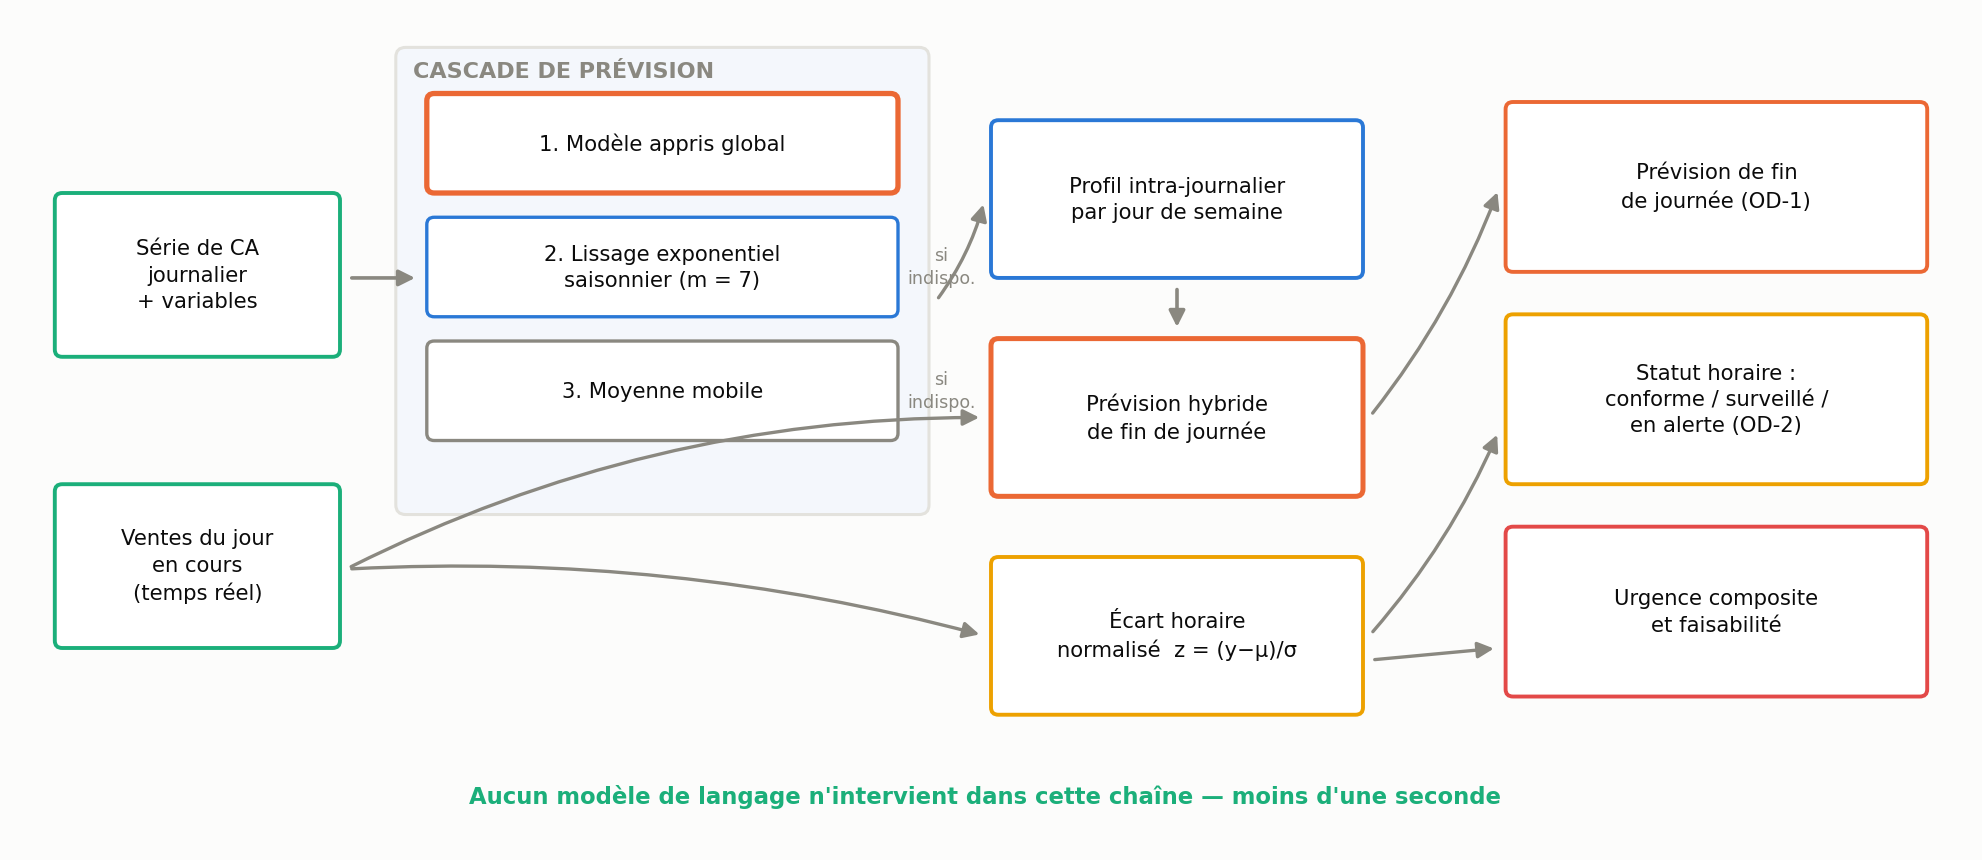
\includegraphics[width=\textwidth]{img/fig_pipeline_prevision_ca.png}
    \caption{Pipeline de prévision du chiffre d'affaires et de détection d'anomalies horaires}
    \label{fig:pipeline-ca-chap4}
\end{figure}

% ------------------------------------------------------------
\section{Modélisation prédictive de la demande}
\label{sec:modele-demande}
% ------------------------------------------------------------

\subsection{Architecture en deux étages}

La prévision de la demande par référence (OD-3) obéit à une architecture en deux étages, motivée par une observation simple : les signaux qui expliquent la demande n'ont pas tous le même horizon de validité. La saisonnalité d'une référence est une propriété lente, estimable sur des mois d'historique et stable d'une semaine à l'autre. Une promotion en cours, un événement à venir ou une rupture récente sont des signaux rapides, dont l'effet se joue sur quelques jours. Vouloir capturer les deux avec un modèle unique conduit soit à noyer les signaux rapides, soit à sur-réagir au bruit.

Le \textbf{premier étage} produit une demande de base par \textbf{décomposition saisonnière multiple}, sur un horizon de trente jours, pour chaque couple référence et point de vente franchissant le seuil d'historique. Cette décomposition sépare la série en tendance, composantes saisonnières et résidu, et projette chaque composante séparément. Elle est recalculée périodiquement plutôt que quotidiennement : la saisonnalité étant une propriété lente, un recalcul quotidien consommerait des ressources considérables sans modifier substantiellement le résultat.

Le \textbf{second étage} applique une \textbf{correction contextuelle} par modèle appris à gradient boosté, sur un horizon de sept jours seulement. Ce modèle ne prédit pas la demande : il prédit l'\textit{écart} entre la demande réelle et la demande de base, à partir des signaux rapides. La borne de sept jours n'est pas arbitraire : au-delà, les variables construites sur le passé récent -- ventes des derniers jours, indicateur de rupture récente -- porteraient sur une fenêtre future dépourvue de données réelles, et le modèle extrapolerait sur ses propres prédictions.

La figure~\ref{fig:pipeline-demande-chap4} présente cette chaîne.

\begin{figure}[H]
    \centering
    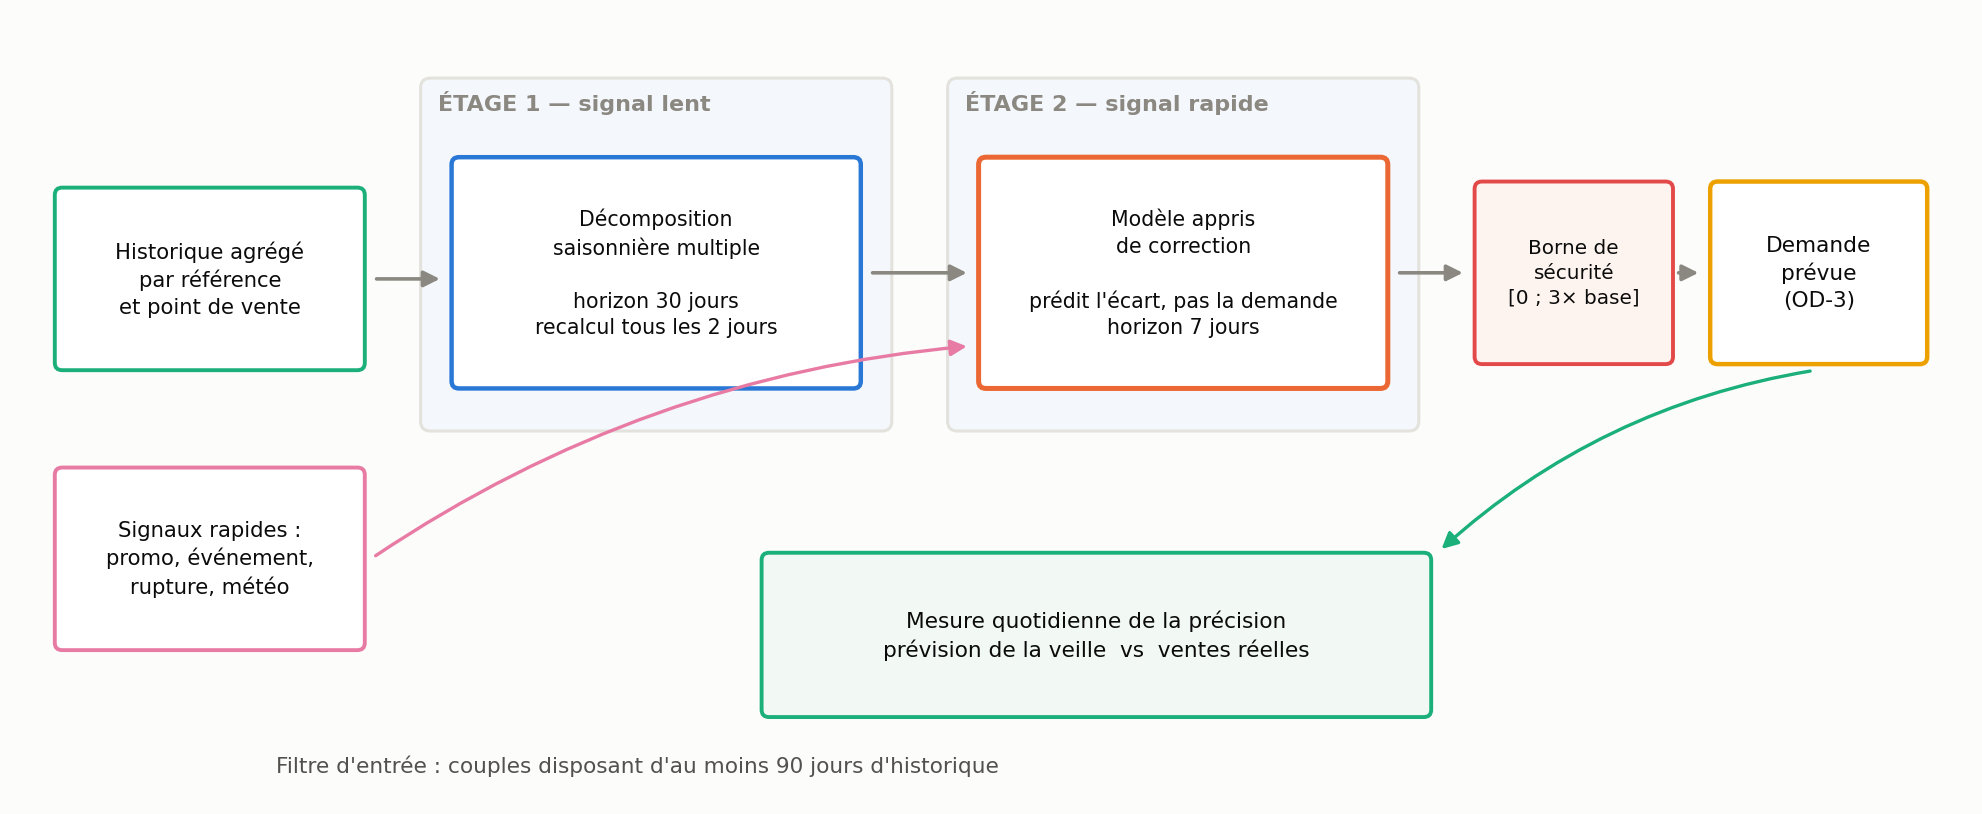
\includegraphics[width=\textwidth]{img/fig_pipeline_prevision_demande.png}
    \caption{Pipeline de prévision de la demande en deux étages}
    \label{fig:pipeline-demande-chap4}
\end{figure}

Une borne de sécurité est appliquée à la sortie du second étage : la demande corrigée est contrainte à rester dans un intervalle proportionnel à la demande de base. Cette borne empêche qu'une combinaison inhabituelle de variables ne produise une valeur extravagante, qui se propagerait ensuite en quantité de commande. C'est une application directe du principe de conception exposé en introduction : le modèle propose une correction, il ne dispose pas de la latitude de produire n'importe quelle valeur.

\subsection{Variables exogènes retenues}

Le tableau~\ref{tab:exogenes-chap4} recense les variables exogènes du second étage et leur justification.

\begingroup
\setlength{\tabcolsep}{3pt}
\renewcommand{\arraystretch}{1.15}
\small

\begin{longtable}{|P{3.4cm}|P{4.0cm}|P{6.1cm}|}
\hline
\rowcolor{red!75}
\textcolor{white}{\textbf{Variable}} &
\textcolor{white}{\textbf{Source}} &
\textcolor{white}{\textbf{Justification}} \\
\hline
\endhead
\hline
\endfoot
\hline
\endlastfoot
Ventes réelles récentes & Historique agrégé & Corrige la dérive de niveau que la base statistique met du temps à intégrer \\
\hline
Promotion active et intensité & Référentiel commercial & Effet fort et de courte durée, structurellement invisible pour la base saisonnière \\
\hline
Événement daté et proximité & Référentiel marché & Un événement local modifie la fréquentation des points de vente voisins uniquement \\
\hline
Indicateur de rupture récente & Historique de stock & Signale que les ventes observées sont censurées et non représentatives de la demande \\
\hline
Conditions météorologiques & Service externe & Module la fréquentation des points de vente physiques \\
\hline
Attributs calendaires & Calcul & Reprennent les effets de cycle de paie et de fin de mois \\
\hline
\caption{Variables exogènes de la couche de correction contextuelle}
\label{tab:exogenes-chap4}
\end{longtable}
\endgroup

\subsection{Boucle de mesure de la précision}

Une composante souvent absente des systèmes de prévision a été intégrée dès la conception : une \textbf{boucle de mesure quotidienne}. Chaque jour, la prévision produite la veille -- de base et corrigée -- est confrontée aux ventes réellement observées, et l'erreur est enregistrée. Cette mesure alimente le suivi de qualité en production décrit au chapitre~\ref{chap:deploiement}, et permet de détecter une dérive du modèle sans attendre un réentraînement.

Cette boucle n'améliore aucune prévision par elle-même. Elle rend le système \textit{observable}, ce qui est une propriété de conception distincte de la performance et tout aussi importante : un modèle dont on ne mesure pas la dérive finit toujours par dériver sans qu'on le sache.

% ------------------------------------------------------------
\section{Modèles de décision de stock}
\label{sec:decision-stock}
% ------------------------------------------------------------

Cette section est la plus déterministe du chapitre, et c'est délibéré : elle porte les calculs qui engagent une commande, donc une dépense. Aucun modèle de langage n'y intervient.

\subsection{Niveau de service et facteur de sécurité}

Le point de départ est le \textbf{niveau de service} cible, c'est-à-dire la probabilité de ne pas connaître de rupture pendant le délai de réapprovisionnement. Ce paramètre n'est pas une grandeur estimée mais une décision de gestion : il traduit l'arbitrage entre le coût d'une rupture et le coût de l'immobilisation. Il est donc fixé par le responsable et non par le système.

Le niveau de service se convertit en \textbf{facteur de sécurité} $z$ par l'inverse de la fonction de répartition de la loi normale centrée réduite, $z = \Phi^{-1}(\mathrm{SL})$. Une table de correspondance sert de repli lorsque le calcul exact n'est pas disponible.

Le niveau de service de base est ajusté selon l'\textbf{étape du cycle de vie} de la référence : relevé pour un produit en lancement ou en croissance, où une rupture compromet le décollage commercial ; abaissé pour un produit en déclin ou en fin de vie, où le risque d'obsolescence dépasse le risque de rupture. Un second ajustement borne le résultat selon l'objectif commercial en vigueur -- maîtrise des coûts, équilibre, priorité au service. Le niveau effectif est enfin contraint à un intervalle admissible, afin qu'aucune combinaison d'ajustements ne conduise à une valeur absurde.

\subsection{Stock de sécurité}

Le stock de sécurité suit la formulation classique tenant compte de la double variabilité, celle de la demande et celle du délai \cite{silver2016inventory,axsater2015inventory} :

\begin{equation}
\mathrm{SS} = z \sqrt{\; \overline{L}\,\sigma_D^2 \;+\; \overline{D}^2\,\sigma_L^2 \;}
\end{equation}

où $\overline{L}$ et $\sigma_L$ désignent la moyenne et l'écart-type du délai de livraison, $\overline{D}$ et $\sigma_D$ la moyenne et l'écart-type de la demande journalière.

La présence du second terme sous le radical mérite d'être commentée, car sa suppression est une erreur fréquente. Ce terme représente la contribution de la \textbf{variabilité du délai fournisseur}. L'ignorer revient à supposer que le fournisseur livre toujours exactement dans le délai annoncé, hypothèse rarement vérifiée. Dans un contexte où les délais sont sujets à aléa, ce terme peut dominer le premier : la principale cause de rupture n'est alors pas une demande exceptionnelle mais une livraison en retard.

L'écart-type de la demande est estimé sur l'historique agrégé par jour, sur une fenêtre glissante. Lorsque l'historique est trop court pour une estimation fiable, une valeur de repli proportionnelle à la demande moyenne est appliquée, et l'observation est tracée comme reposant sur un repli.

\subsection{Point de commande}

Le point de commande, seuil en dessous duquel une commande doit être déclenchée, est la somme de la demande attendue pendant le délai et du stock de sécurité :

\begin{equation}
\mathrm{ROP} = \overline{D} \times \overline{L} + \mathrm{SS}
\end{equation}

\subsection{Quantité économique de commande}

La quantité commandée suit la formulation économique classique \cite{harris1913eoq}, qui minimise la somme du coût de passation et du coût de possession :

\begin{equation}
\mathrm{EOQ} = \sqrt{\frac{2\, D_{\text{annuelle}}\, C_p}{h\, C_u}}
\end{equation}

où $C_p$ est le coût fixe de passation d'une commande, $C_u$ le coût unitaire de la référence et $h$ le taux annuel de coût de possession.

Cette formule repose sur des hypothèses fortes -- demande constante, délai constant, absence de remise sur quantité -- qui ne sont jamais exactement vérifiées. Elle est néanmoins retenue, pour une raison assumée : elle fournit un ordre de grandeur défendable et explicable, ce qu'aucune heuristique arbitraire ne procure. La quantité obtenue est ensuite ajustée aux \textbf{contraintes fournisseurs} : arrondi au conditionnement, respect de la quantité minimale de commande, plafonnement par la capacité de stockage. Ce sont ces contraintes, et non la formule, qui déterminent souvent la quantité finale.

La sensibilité de cette quantité à la qualité du paramétrage -- limite identifiée au chapitre~\ref{chap:donnees} -- est mesurée séparément au chapitre~\ref{chap:evaluation}.

\subsection{Classification du risque}

La classification du risque (OD-4) procède en deux couches, la plus sévère l'emportant.

La \textbf{première couche} applique les seuils de gestion définis par le responsable. Si le stock total, disponible et en transit, est inférieur ou égal au seuil minimal, la référence est classée en risque critique. S'il dépasse le seuil maximal, un indicateur de surstock est levé.

La \textbf{seconde couche} raisonne par la couverture rapportée au délai. Soit $d$ le nombre de jours de couverture restants :

\begin{itemize}[label=--]
    \item $d < \overline{L}$ : risque critique -- le stock s'épuisera avant l'arrivée de la prochaine commande ;
    \item $\overline{L} \le d < \overline{L} + 2\sigma_L$ : risque élevé -- le stock tombe dans la fenêtre de variabilité du délai ;
    \item $\overline{L} + 2\sigma_L \le d < 2{,}5\,\overline{L}$ : risque moyen ;
    \item $d \ge 2{,}5\,\overline{L}$ : risque faible.
\end{itemize}

La justification de cette double couche tient à la nature différente des deux informations. Les seuils de gestion encodent une connaissance que le calcul ignore : contrainte contractuelle, importance stratégique d'une référence, contrainte d'exposition en rayon. Le calcul par la couverture, lui, s'adapte automatiquement à l'évolution de la demande et du délai. Retenir la plus sévère des deux revient à ne jamais laisser un calcul contredire une décision de gestion explicite, tout en conservant la réactivité du calcul. La bimodalité de la couverture observée au chapitre~\ref{chap:donnees} justifie par ailleurs la levée séparée de l'indicateur de surstock : le risque n'est pas unidimensionnel.

\subsection{Arbre de décision}

La décision finale résulte de l'arbre présenté en figure~\ref{fig:arbre-decision-chap4}.

\begin{figure}[H]
    \centering
    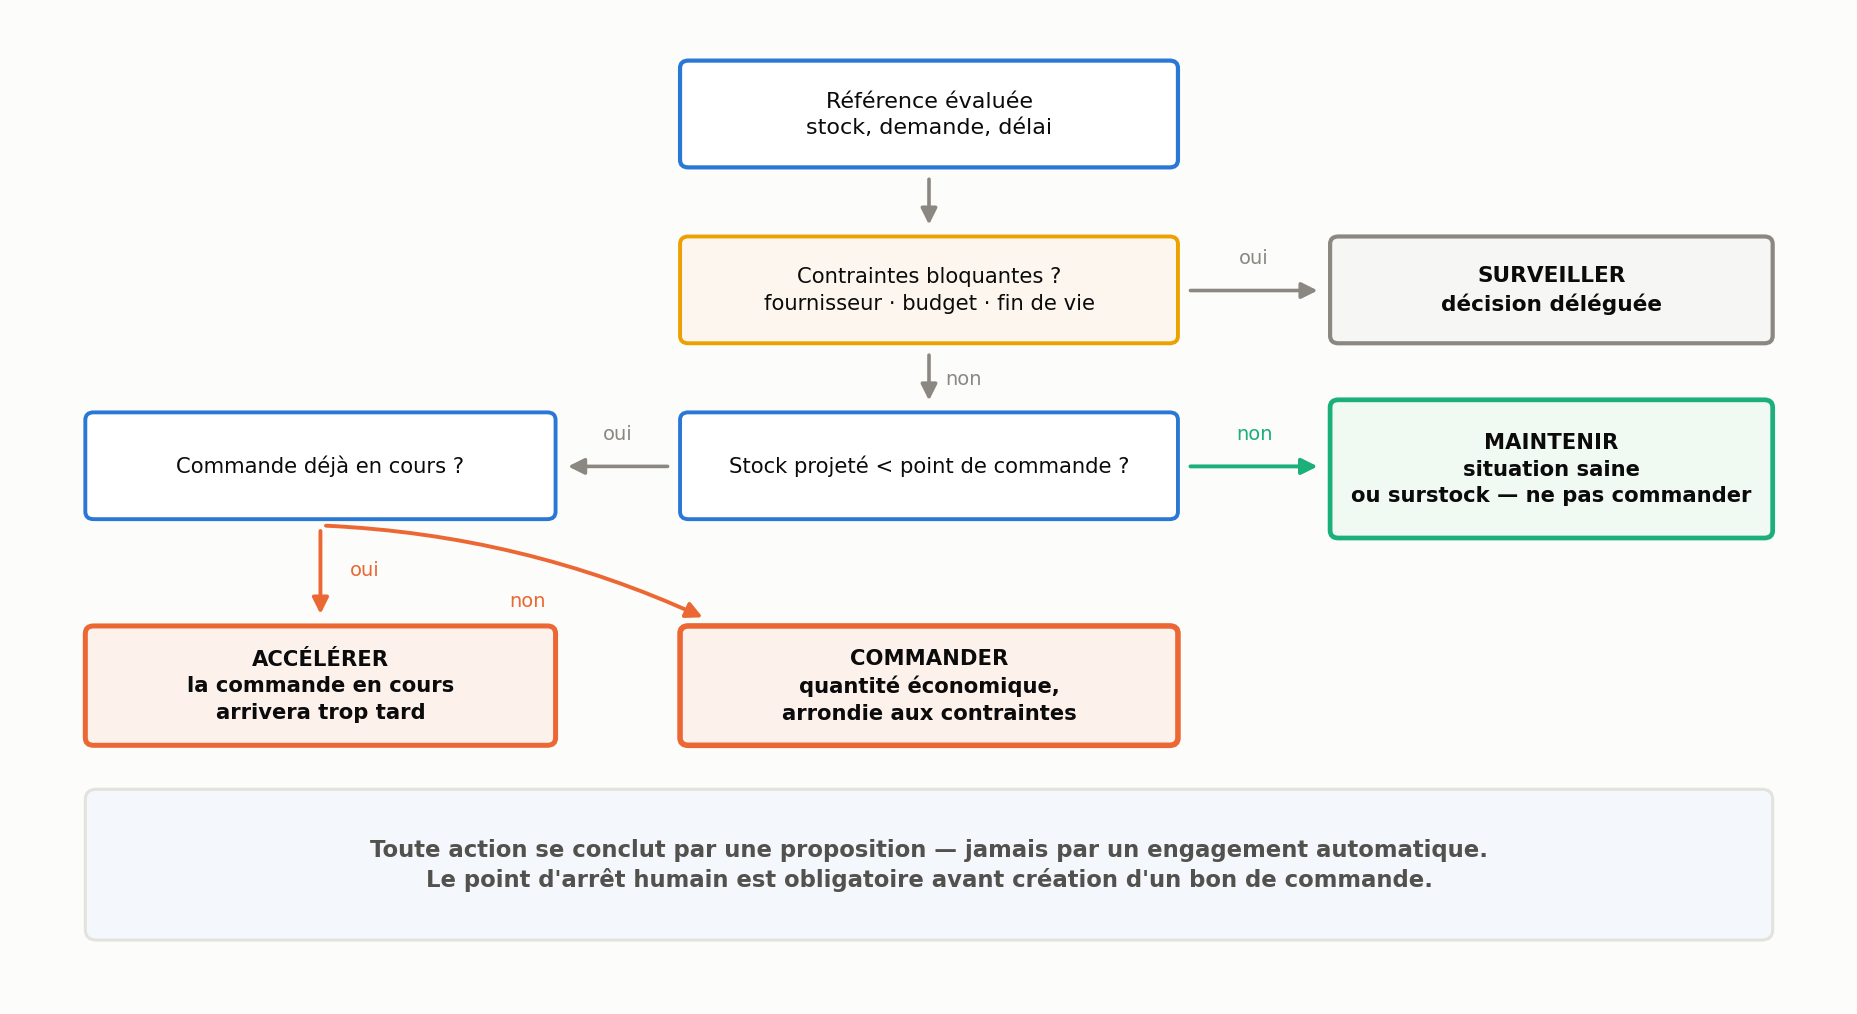
\includegraphics[width=\textwidth]{img/fig_arbre_decision_stock.png}
    \caption{Arbre de décision de réapprovisionnement}
    \label{fig:arbre-decision-chap4}
\end{figure}

Quatre actions sont possibles. \textbf{Commander} lorsque le stock projeté franchit le point de commande et qu'aucune contrainte ne s'y oppose. \textbf{Accélérer} lorsqu'une commande est déjà en cours mais arrivera trop tard au regard de la couverture restante -- action qui n'a de sens que parce que le système connaît l'état des commandes en cours, et qui illustre l'intérêt d'avoir intégré le domaine de l'approvisionnement. \textbf{Maintenir} lorsque la situation est saine ou en surstock, décision explicite et non simple absence de décision. \textbf{Surveiller} lorsque les signaux sont contradictoires ou les données insuffisantes pour trancher, cas dans lequel la décision est déléguée à l'humain plutôt que forcée.

L'existence de cette quatrième branche est un choix de conception important. Un système qui tranche toujours donne une impression de compétence mais produit nécessairement des décisions arbitraires sur les cas ambigus. Reconnaître explicitement l'ambiguïté et la remonter est préférable, à condition que le volume de cas ainsi remontés reste maîtrisé -- ce que le chapitre~\ref{chap:evaluation} vérifie.

% ------------------------------------------------------------
\section{Conception des agents intelligents}
\label{sec:agents}
% ------------------------------------------------------------

Le système compte huit agents répartis sur les deux domaines métier, coordonnés par un méta-orchestrateur. Chaque agent est conçu comme un graphe d'états dont les nœuds sont des étapes de traitement, conformément au cadre d'orchestration retenu au chapitre~\ref{chap:comprehension-metier}. Le tableau~\ref{tab:agents-chap4} en donne la vue d'ensemble.

\begingroup
\setlength{\tabcolsep}{3pt}
\renewcommand{\arraystretch}{1.15}
\small

\begin{longtable}{|P{2.1cm}|P{1.5cm}|P{4.3cm}|P{4.0cm}|P{1.5cm}|}
\hline
\rowcolor{red!75}
\textcolor{white}{\textbf{Agent}} &
\textcolor{white}{\textbf{Domaine}} &
\textcolor{white}{\textbf{Rôle}} &
\textcolor{white}{\textbf{Sortie principale}} &
\textcolor{white}{\textbf{Génératif}} \\
\hline
\endhead
\hline
\endfoot
\hline
\endlastfoot
Analyste & Ventes & Prévision, écart, urgence, faisabilité & Diagnostic chiffré de la journée & Non \\
\hline
Stratège & Ventes & Cause racine et plan d'action commercial & Actions priorisées et produits cibles & Oui \\
\hline
Coach & Ventes & Dialogue avec le conseiller & Réponse conversationnelle ancrée & Oui \\
\hline
Garde-fou & Ventes & Contrôle de conformité de la recommandation & Verdict et motifs & Non \\
\hline
Analyse & Stocks & Métriques de stock et classification du risque & Rapport d'analyse par référence & Partiel \\
\hline
Contexte & Stocks & Effet attendu des événements et promotions & Coefficient de correction de demande & Oui \\
\hline
Décision & Stocks & Action de réapprovisionnement & Décision, quantité, justification & Oui \\
\hline
Fusion cross-domaine & Transverse & Hiérarchisation des produits à proposer & Liste ordonnée et scores & Non \\
\hline
Superviseur & Méta & Orchestration de l'ensemble & État consolidé du cycle & Non \\
\hline
\caption{Rôle et nature de chaque agent du système}
\label{tab:agents-chap4}
\end{longtable}
\endgroup

La colonne « génératif » de ce tableau constitue une lecture directe du principe de conception : cinq des neuf unités n'invoquent aucun modèle de langage. L'agent Analyste, qui porte pourtant l'essentiel de la valeur analytique du domaine Ventes, en est totalement dépourvu.

\subsection{Agent Analyste}

L'agent Analyste enchaîne sept étapes : réception des données de caisse, validation, chargement de la mémoire du cycle précédent, appel au moteur de séries temporelles décrit en section~\ref{sec:modele-ca}, comparaison à l'état précédent, construction de la requête destinée au Stratège, et sauvegarde de la mémoire.

L'étape de construction de la requête est ce qui impose le séquencement entre Analyste et Stratège : le second consomme une formulation produite par le premier. Cette dépendance de données, et non une préférence de conception, est ce qui interdit de les exécuter en parallèle.

L'étape de comparaison à la mémoire mérite également d'être signalée. Elle permet de qualifier l'évolution -- la situation s'améliore-t-elle ou se dégrade-t-elle depuis le cycle précédent ? -- information qu'aucune analyse instantanée ne peut produire et qui change pourtant complètement le conseil à formuler.

\subsection{Agent Stratège}

L'agent Stratège enchaîne six étapes : collecte du contexte externe, recherche documentaire, analyse du contexte, génération de la stratégie, mise en forme, et auto-critique.

La dernière étape implémente le patron de \textbf{réflexion} \cite{yao2023react} : l'agent relit sa propre production et l'évalue sur des critères de cohérence et de complétude, produisant un score de confiance. Ce score n'est pas décoratif : il alimente l'une des règles du contrôle de conformité décrit en section~\ref{sec:conformite}, de sorte qu'une stratégie que l'agent lui-même juge peu assurée sera escaladée vers un humain plutôt que diffusée.

\subsection{Agent Coach}

L'agent Coach est le plus complexe du système car il opère en dialogue. Son traitement enchaîne la classification de l'intention du message, le chargement parallèle des contextes pertinents, une recherche documentaire couvrant les deux domaines, la sollicitation du Stratège, la recherche de substituts en cas de mention d'un produit indisponible, et enfin la génération de la réponse.

Deux mécanismes méritent d'être détaillés.

Le premier est la \textbf{hiérarchie de sources} imposée par la consigne système. Les informations dont dispose le Coach proviennent de natures très différentes : chiffres calculés par les agents, extraits documentaires, fiches produit, décisions passées. En cas de contradiction, l'ordre de priorité est explicitement fixé, les productions des agents et les chiffres primant sur les extraits documentaires. Sans cette hiérarchie, un script de vente générique pourrait contredire un chiffre calculé, et le modèle n'aurait aucun moyen de trancher.

Le second est le mécanisme de \textbf{substitution}. Lorsque le conseiller mentionne un produit en rupture, le Coach ne se contente pas de le signaler : il propose des substituts effectivement disponibles, sélectionnés par requête sur la gamme et le positionnement tarifaire, puis ordonnés par le score de fusion. Ce mécanisme traite directement la première cause d'inutilité d'un assistant commercial : recommander ce qui n'est pas vendable.

\subsection{Fusion cross-domaine et score produit}

La hiérarchisation des produits à proposer (OD-6) repose sur un score multicritère combinant six dimensions, dont trois relèvent du domaine Ventes et trois du domaine Stocks :

\begin{equation}
\begin{split}
S = \; & 0{,}30\, a_{\text{gap}} + 0{,}20\, a_{\text{stock}} + 0{,}15\, a_{\text{marge}} \\
       & + 0{,}15\, a_{\text{promo}} + 0{,}10\, a_{\text{conseiller}} + 0{,}10\, a_{\text{client}}
\end{split}
\end{equation}

où chaque composante $a_i$ est normalisée dans l'intervalle $[0,1]$ et calculée dynamiquement à partir des données, sans valeur figée dans le code.

La composante $a_{\text{gap}}$ mesure l'adéquation du prix du produit à l'écart de chiffre d'affaires restant à combler : proposer un accessoire lorsqu'il manque plusieurs milliers de dinars est inopérant, proposer un terminal haut de gamme lorsqu'il manque le prix d'une recharge l'est tout autant. La composante $a_{\text{stock}}$ traduit la santé du stock. Les composantes $a_{\text{marge}}$ et $a_{\text{promo}}$ portent la priorité commerciale. Les composantes $a_{\text{conseiller}}$ et $a_{\text{client}}$ personnalisent le classement selon la performance historique du conseiller sur la catégorie et selon le profil de conversion du produit.

Le poids dominant accordé à l'adéquation au gap traduit une décision métier explicite : la finalité du conseil est de combler l'écart à l'objectif, les autres critères modulant ce choix sans le renverser. La figure~\ref{fig:correlation-chap4} rappelle pourquoi ce score composite est nécessaire plutôt qu'un tri simple.

\begin{figure}[H]
    \centering
    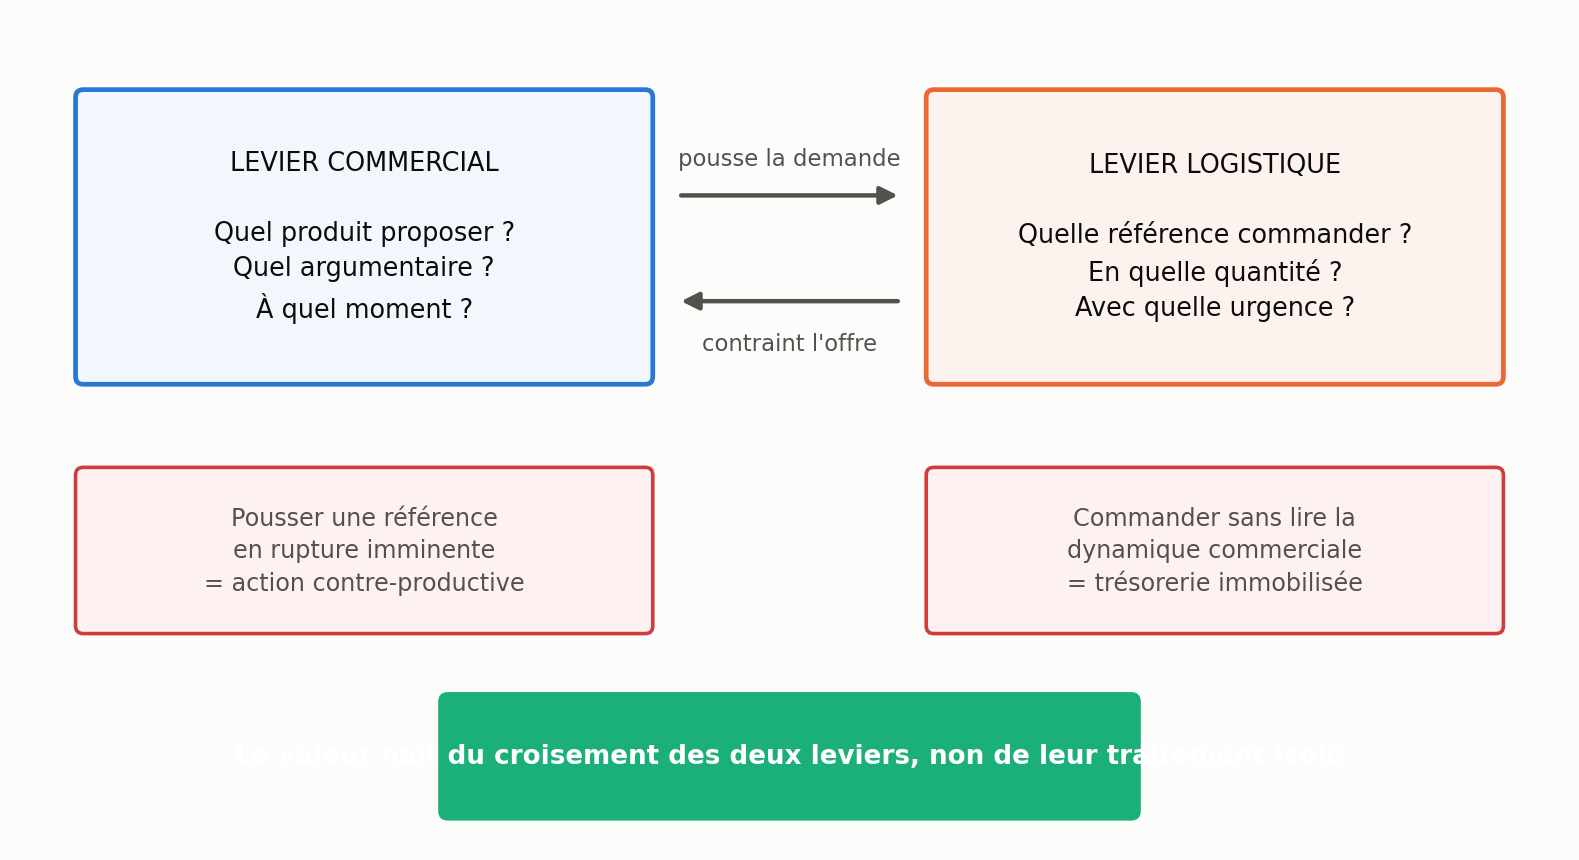
\includegraphics[width=0.9\textwidth]{img/fig_couplage_domaines.png}
    \caption{Couplage des domaines Ventes et Stocks dans le score produit}
    \label{fig:correlation-chap4}
\end{figure}

La sortie du score n'est pas seulement une valeur mais le \textbf{détail de ses composantes}. Cette décomposition est ce qui rend la recommandation explicable : le conseiller peut voir qu'un produit est proposé parce que sa marge est élevée et son stock sain, non parce qu'un modèle opaque en a décidé ainsi.

\subsection{Chaîne du domaine Stocks}

Le domaine Stocks mobilise trois agents selon un enchaînement où deux d'entre eux s'exécutent en parallèle. L'agent \textbf{Analyse} calcule les métriques de la section~\ref{sec:decision-stock} et classe le risque ; le modèle de langage n'y intervient qu'en évaluateur, pour arbitrer les cas où les dimensions du diagnostic se contredisent. L'agent \textbf{Contexte} estime l'effet attendu des événements et promotions à venir, par apprentissage des effets observés lors d'occurrences passées comparables. L'agent \textbf{Décision} fusionne les deux, applique la correction de demande, vérifie les contraintes, et produit l'action et sa justification.

Une propriété de conception de l'agent Décision mérite d'être soulignée : lorsque la vérification des contraintes conclut à l'impossibilité de commander -- fournisseur indisponible, budget épuisé, référence en fin de vie --, le traitement s'arrête sans solliciter le modèle de langage. Il serait absurde de faire rédiger la justification d'une commande qui ne peut pas être passée.

% ------------------------------------------------------------
\section{Base de connaissances métier et recherche hybride}
\label{sec:rag}
% ------------------------------------------------------------

L'objectif OD-7 vise à retrouver l'argumentaire pertinent dans la connaissance métier de l'entreprise. Il est traité par un mécanisme de génération augmentée par la recherche \cite{lewis2020rag,gao2024rag}, dont la figure~\ref{fig:pipeline-rag-chap4} présente la chaîne.

\begin{figure}[H]
    \centering
    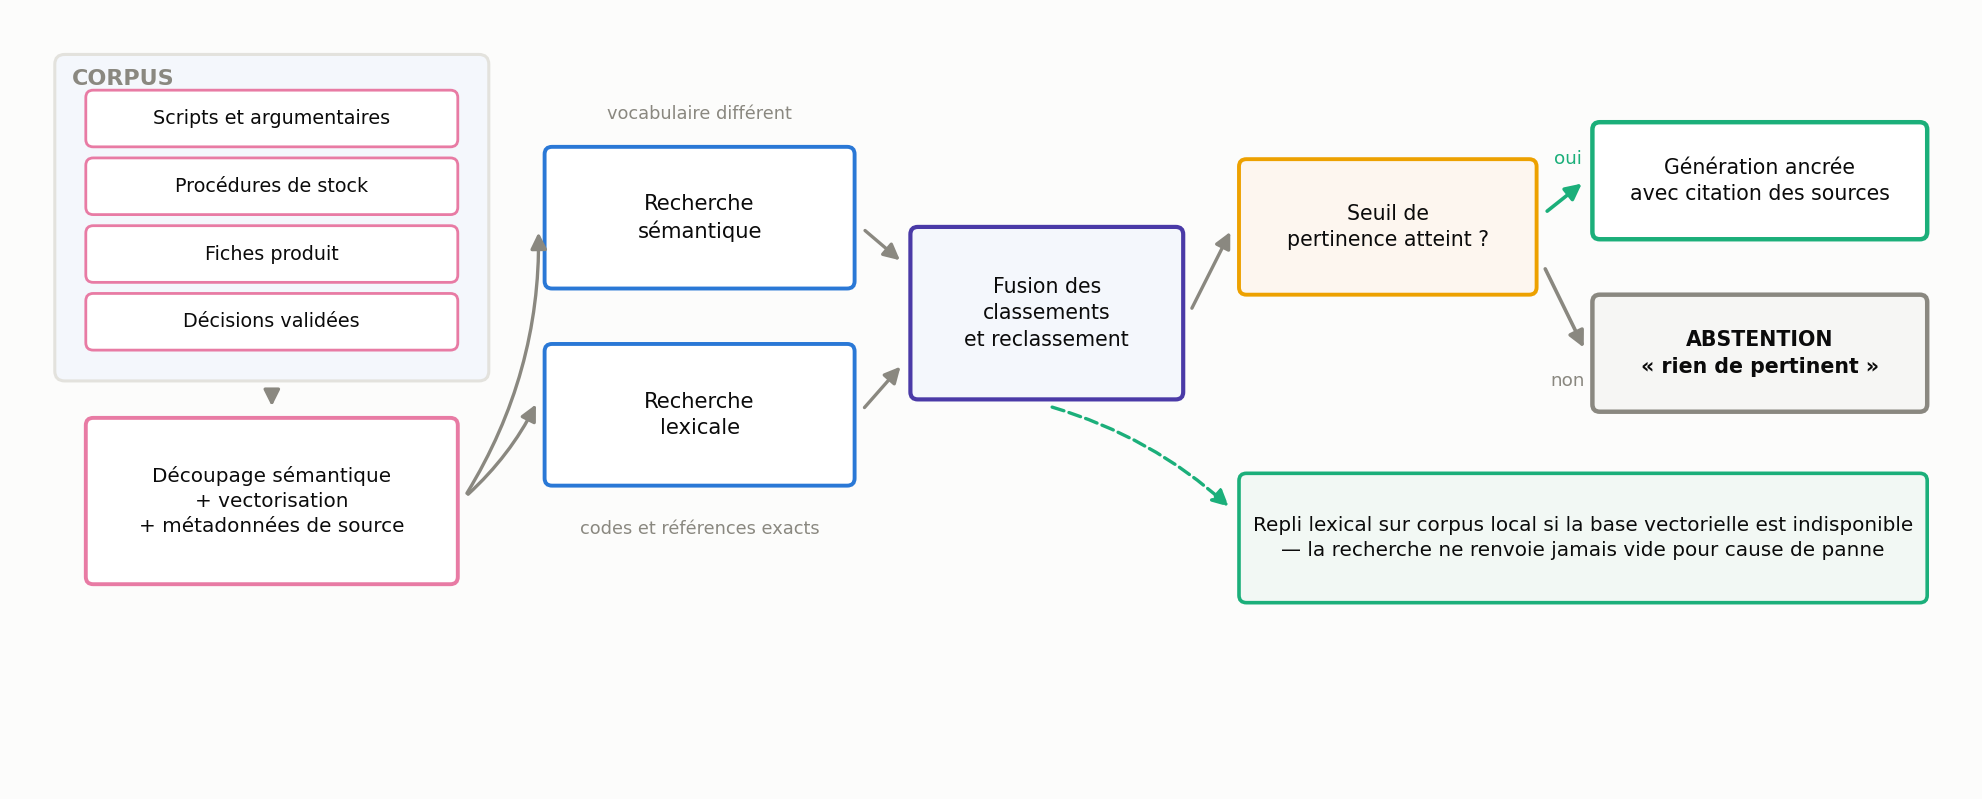
\includegraphics[width=\textwidth]{img/fig_pipeline_rag.png}
    \caption{Chaîne de recherche documentaire hybride et de génération ancrée}
    \label{fig:pipeline-rag-chap4}
\end{figure}

\subsection{Constitution et découpage du corpus}

Le corpus rassemble quatre familles de documents : scripts de vente et argumentaires, procédures et guides opératoires du domaine des stocks, fiches produit, et historique des décisions validées. Cette dernière famille est particulière : elle se constitue au fil de l'exploitation, chaque interaction validée venant enrichir le corpus. Le système apprend ainsi de ses propres décisions passées sans réentraînement de modèle.

Le découpage suit les frontières sémantiques des documents plutôt qu'une longueur fixe, afin qu'un extrait retrouvé constitue une unité de sens complète. Chaque extrait conserve les métadonnées permettant de le rattacher à sa source, condition nécessaire à la citation exigée par le critère de succès d'OD-7.

\subsection{Recherche hybride}

La recherche combine deux modalités complémentaires. La \textbf{recherche sémantique} compare la représentation vectorielle de la requête à celle des extraits, ce qui permet de retrouver un contenu pertinent formulé avec un vocabulaire différent. La \textbf{recherche lexicale}, fondée sur une pondération de type fréquence-rareté \cite{robertson2009bm25}, retrouve les correspondances exactes de termes.

La complémentarité des deux est ce qui justifie l'hybridation, et elle s'observe précisément sur ce corpus. Les références produit, les codes d'offre et les termes techniques sont des chaînes que la recherche lexicale retrouve exactement et que la recherche sémantique dilue. Inversement, une question formulée en langage courant sur un besoin client ne partage aucun terme avec l'argumentaire pertinent, que seule la recherche sémantique retrouve. Les deux classements sont fusionnés, puis les extraits sont ordonnés selon leur pertinence conjointe.

\subsection{Mécanisme de repli}

La base vectorielle est un composant externe, susceptible d'être indisponible. Un mécanisme de repli sur un corpus local, interrogé lexicalement, garantit que la recherche ne renvoie jamais un résultat vide pour cause de panne d'infrastructure. Cette précaution répond à l'exigence non fonctionnelle de robustesse : une indisponibilité de composant doit dégrader la qualité du service, non l'interrompre.

Un second garde-fou porte sur la pertinence. Lorsque aucun extrait ne dépasse le seuil de pertinence, la chaîne le signale explicitement plutôt que de transmettre les extraits les moins mauvais. Cette capacité d'\textbf{abstention} est ce qui distingue une chaîne documentaire fiable d'une chaîne qui produit une réponse plausible en toute circonstance -- c'est-à-dire qui hallucine \cite{ji2023hallucination}.

% ------------------------------------------------------------
\section{Orchestration multi-agents}
\label{sec:orchestration}
% ------------------------------------------------------------

\subsection{État partagé et communication entre agents}

Les agents ne s'appellent jamais directement. Toute communication transite par un \textbf{état partagé} unique, que chaque agent lit et enrichit. Ce choix architectural, caractéristique des systèmes multi-agents à coordination par tableau noir \cite{wooldridge2009mas}, présente trois avantages : chaque agent est testable isolément en lui fournissant un état de départ ; un agent peut être remplacé sans modifier les autres ; et le parallélisme devient possible dès lors que les agents concurrents écrivent dans des champs distincts.

Cette dernière condition n'est pas automatiquement satisfaite et sa violation a constitué l'une des difficultés notables du projet. Lorsque plusieurs agents s'exécutent simultanément et écrivent dans le même champ, le cadre d'orchestration ne peut déterminer quelle valeur retenir. Deux mécanismes complémentaires résolvent ce problème.

Le premier est la règle selon laquelle \textbf{chaque étape ne retourne que ce qu'elle produit}, et non l'état complet. Retourner l'état complet -- réflexe naturel -- fait apparaître chaque agent comme écrivant dans tous les champs, y compris ceux qu'il s'est contenté de lire, provoquant des conflits sur des champs qu'il ne modifie pourtant pas.

Le second est la définition de \textbf{fonctions de fusion} pour les champs légitimement écrits par plusieurs branches : concaténation pour les listes d'agents mobilisés et d'erreurs, fusion pour les dictionnaires de métriques. Ces fonctions rendent l'écriture concurrente déterministe.

Le tableau~\ref{tab:proprietaires-chap4} présente la répartition des champs par branche propriétaire, qui garantit par construction l'absence de conflit sur les champs restants.

\begingroup
\setlength{\tabcolsep}{3pt}
\renewcommand{\arraystretch}{1.15}
\small

\begin{longtable}{|P{3.2cm}|P{10.5cm}|}
\hline
\rowcolor{red!75}
\textcolor{white}{\textbf{Branche}} &
\textcolor{white}{\textbf{Champs dont elle est seule propriétaire}} \\
\hline
\endhead
\hline
\endfoot
\hline
\endlastfoot
Ventes & Écart, urgence, faisabilité, synthèse analytique, stratégie et actions, produits focus, écarts horaires, analyse temporelle \\
\hline
Connaissance & Contexte documentaire, extraits retrouvés \\
\hline
Contexte & Contexte externe, rapport de contexte \\
\hline
Stocks & Décisions de réapprovisionnement, alertes de stock critiques \\
\hline
Coach & Recommandation au conseiller, produits scorés \\
\hline
Garde-fou & Statut de conformité, motifs, retour, exigence de validation humaine \\
\hline
\caption{Répartition des champs de l'état partagé par branche propriétaire}
\label{tab:proprietaires-chap4}
\end{longtable}
\endgroup

\subsection{Graphe d'orchestration}

La figure~\ref{fig:graphe-orchestration-chap4} présente le graphe du superviseur.

\begin{figure}[H]
    \centering
    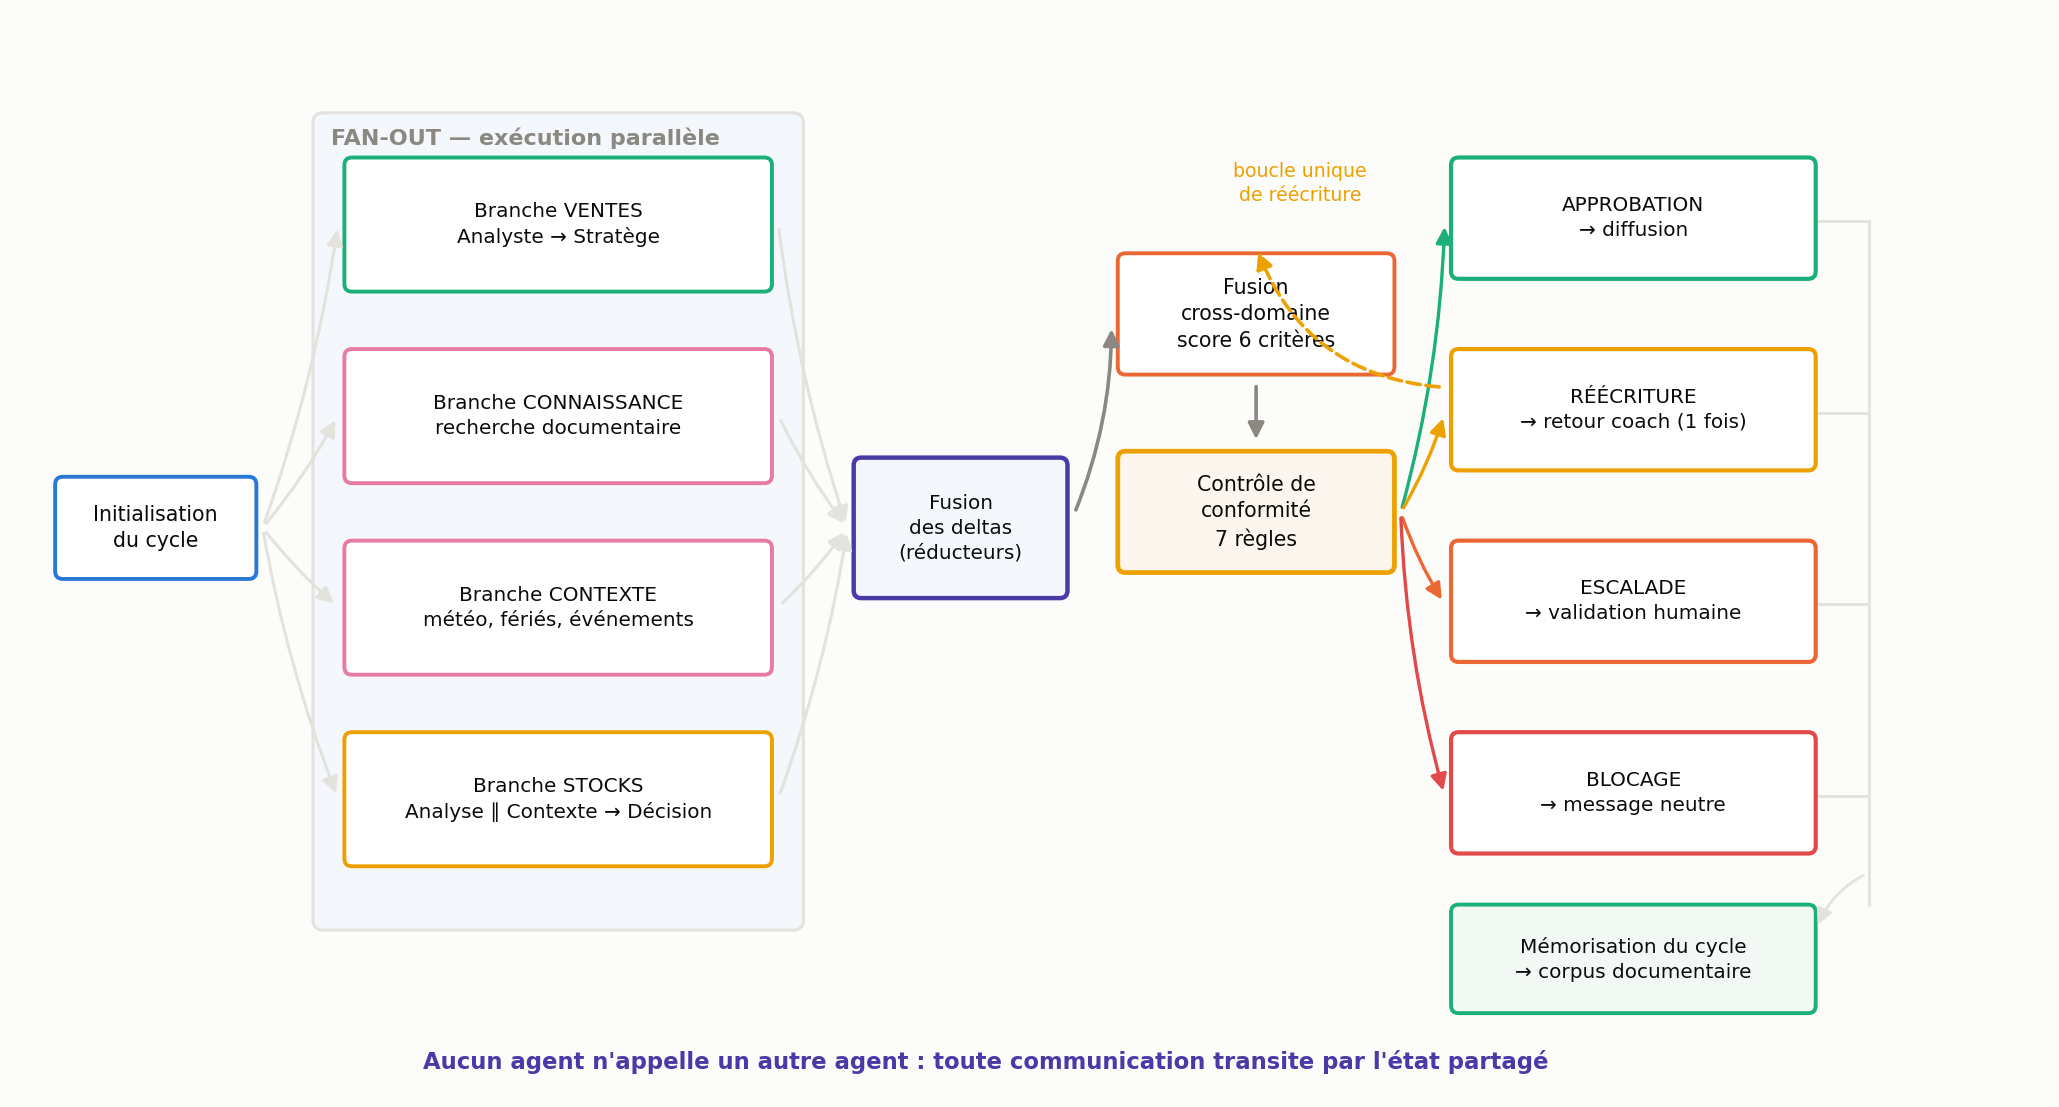
\includegraphics[width=\textwidth]{img/fig_graphe_orchestration.png}
    \caption{Graphe d'orchestration multi-agents : divergence parallèle, convergence et routage conditionnel}
    \label{fig:graphe-orchestration-chap4}
\end{figure}

Le graphe procède en trois temps. Une \textbf{divergence} lance quatre branches en parallèle : ventes, connaissance, contexte et stocks. Une \textbf{convergence} fusionne leurs productions dans l'état partagé. Une \textbf{séquence de décision} enchaîne ensuite la fusion cross-domaine, le contrôle de conformité, et le routage selon le verdict.

Le choix entre exécution parallèle et séquentielle est dicté par les dépendances de données réelles et non par une préférence de performance. Les quatre branches sont parallèles parce qu'aucune ne consomme la production d'une autre. À l'intérieur de la branche Ventes, Analyste et Stratège sont séquentiels en raison de la dépendance décrite en section~\ref{sec:agents}. Dans la branche Stocks, Analyse et Contexte sont parallèles et Décision les fusionne.

\subsection{Déclencheurs}

Trois voies déclenchent un cycle, présentées au tableau~\ref{tab:declencheurs-chap4}.

\begingroup
\setlength{\tabcolsep}{3pt}
\renewcommand{\arraystretch}{1.15}
\small

\begin{longtable}{|P{2.9cm}|P{2.6cm}|P{8.2cm}|}
\hline
\rowcolor{red!75}
\textcolor{white}{\textbf{Déclencheur}} &
\textcolor{white}{\textbf{Rythme}} &
\textcolor{white}{\textbf{Traitement}} \\
\hline
\endhead
\hline
\endfoot
\hline
\endlastfoot
Cycle périodique & Quart d'heure & Cycle complet sur les points de vente les plus actifs \\
\hline
Événement de vente & À la transaction, avec temporisation & Deux étages : analyse déterministe seule d'abord ; cycle complet uniquement si l'urgence progresse, si l'écart franchit un seuil ou si la faisabilité se dégrade \\
\hline
Alerte de stock & À l'apparition d'une rupture & Cycle complet immédiat, avec temporisation pour éviter les rafales \\
\hline
Requête utilisateur & À la demande & Chaîne du Coach uniquement \\
\hline
\caption{Déclencheurs de cycle et traitement associé}
\label{tab:declencheurs-chap4}
\end{longtable}
\endgroup

Le déclencheur sur événement de vente, avec ses deux étages, illustre un compromis de conception significatif. Déclencher un cycle complet à chaque vente serait à la fois inutile -- la plupart des ventes ne changent rien au diagnostic -- et coûteux, chaque cycle mobilisant plusieurs appels à des modèles de langage facturés. N'en déclencher aucun ferait perdre la réactivité qui fait tout l'intérêt du temps réel. Le premier étage, purement déterministe et donc gratuit et instantané, recalcule le diagnostic ; le second étage, coûteux, n'est engagé que si le diagnostic a matériellement changé.

% ------------------------------------------------------------
\section{Contrôle de conformité et validation humaine}
\label{sec:conformite}
% ------------------------------------------------------------

\subsection{Règles de conformité}

Toute recommandation destinée à un utilisateur traverse un contrôle de conformité avant diffusion. Ce contrôle applique sept règles déterministes, présentées au tableau~\ref{tab:guardrails-chap4}.

\begingroup
\setlength{\tabcolsep}{3pt}
\renewcommand{\arraystretch}{1.15}
\small

\begin{longtable}{|P{1.1cm}|P{3.0cm}|P{6.6cm}|P{2.6cm}|}
\hline
\rowcolor{red!75}
\textcolor{white}{\textbf{Réf.}} &
\textcolor{white}{\textbf{Objet}} &
\textcolor{white}{\textbf{Contrôle}} &
\textcolor{white}{\textbf{Verdict}} \\
\hline
\endhead
\hline
\endfoot
\hline
\endlastfoot
G1 & Disponibilité & Aucun produit à stock nul ne peut être recommandé & Blocage \\
\hline
G2 & Rupture imminente & Un produit dont la couverture est très courte n'est pas poussé, sauf intention explicite de déstockage & Réécriture \\
\hline
G3 & Ancrage & Un argument commercial doit provenir d'une source identifiée lorsque la confiance est faible & Réécriture \\
\hline
G4 & Engagement commercial & Aucune remise ni offre non autorisée ne peut être formulée & Blocage \\
\hline
G5 & Éligibilité technique & Aucun service soumis à condition d'éligibilité ne peut être promis sans vérification & Réécriture \\
\hline
G6 & Confiance & Une recommandation dont la confiance est insuffisante est soumise à relecture humaine & Escalade \\
\hline
G7 & Engagement financier & Toute commande dépassant le seuil défini requiert une validation hiérarchique & Escalade \\
\hline
\caption{Règles de contrôle de conformité et verdict associé}
\label{tab:guardrails-chap4}
\end{longtable}
\endgroup

Le verdict global est la sévérité maximale parmi les règles violées. Ce choix, plutôt qu'une moyenne ou un vote, traduit la nature du contrôle : une seule violation bloquante suffit à interdire la diffusion, quel que soit le nombre de règles respectées par ailleurs.

\subsection{Automate de verdicts}

La figure~\ref{fig:automate-guardrail-chap4} présente l'automate de routage.

\begin{figure}[H]
    \centering
    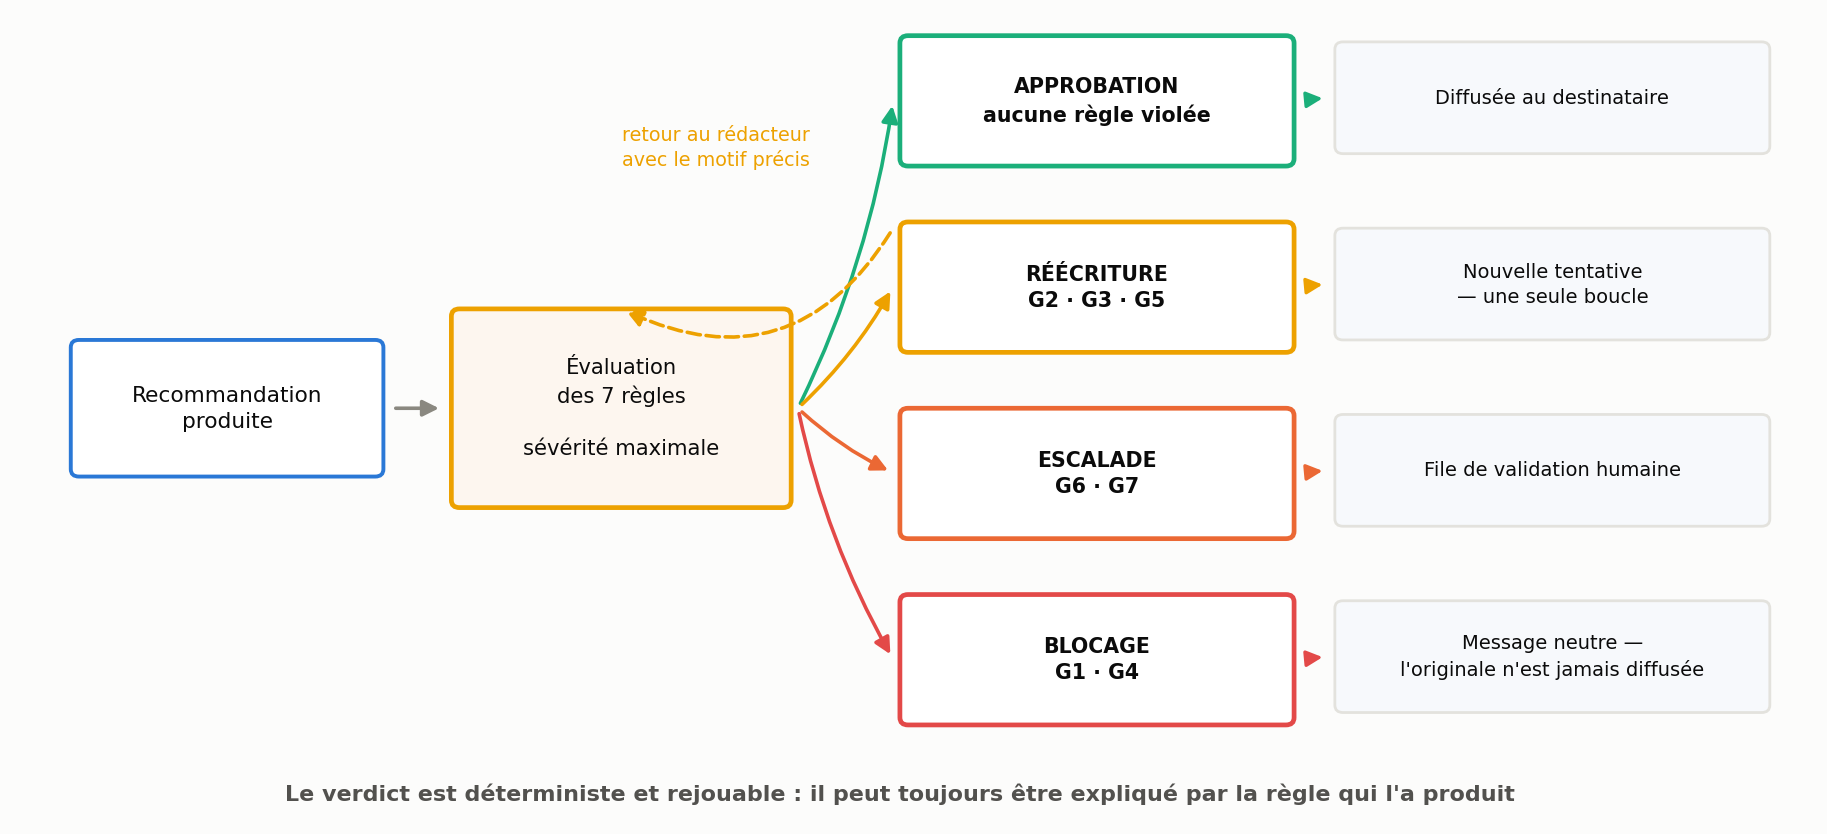
\includegraphics[width=\textwidth]{img/fig_automate_guardrail.png}
    \caption{Automate d'états du contrôle de conformité}
    \label{fig:automate-guardrail-chap4}
\end{figure}

Quatre issues sont possibles. L'\textbf{approbation} transmet la recommandation telle quelle. La \textbf{réécriture} renvoie la recommandation à son auteur, accompagnée du motif précis de non-conformité, pour une nouvelle tentative -- limitée à une seule boucle, afin qu'un désaccord persistant ne produise pas une oscillation infinie. L'\textbf{escalade} place la recommandation dans une file de validation humaine. Le \textbf{blocage} substitue un message neutre à la recommandation, l'originale n'étant jamais transmise.

Cette architecture réalise deux niveaux d'auto-correction imbriqués. Le premier est interne au Stratège, par son étape d'auto-critique. Le second est externe, du contrôle de conformité vers le Coach. Les deux sont chaînés : le score de confiance produit par l'auto-critique alimente la règle G6.

\subsection{Point d'arrêt et validation humaine}

Aucun engagement -- commande, envoi d'une recommandation escaladée -- n'est effectué sans décision humaine. Le graphe s'interrompt à un point d'arrêt explicite, l'état du cycle est persisté, et l'exécution reprend lorsque la décision est rendue. Cette conception suit les recommandations en matière d'interaction humain-intelligence artificielle \cite{amershi2019guidelines,mosqueira2023human} : le système propose, l'humain dispose, et la reprise après décision ne perd aucun contexte.

Le retour humain n'est pas seulement une porte : il est \textbf{capturé}. L'acceptation ou le refus, et dans ce dernier cas le motif, sont enregistrés et rattachés à la recommandation d'origine. Ces données alimentent d'une part le tableau de supervision décrit au chapitre~\ref{chap:deploiement}, d'autre part le corpus documentaire, de sorte que les décisions validées deviennent une source de connaissance pour les cycles suivants.

\subsection{Cycle de vie du bon de commande}

La figure~\ref{fig:cycle-po-chap4} présente l'automate du bon de commande.

\begin{figure}[H]
    \centering
    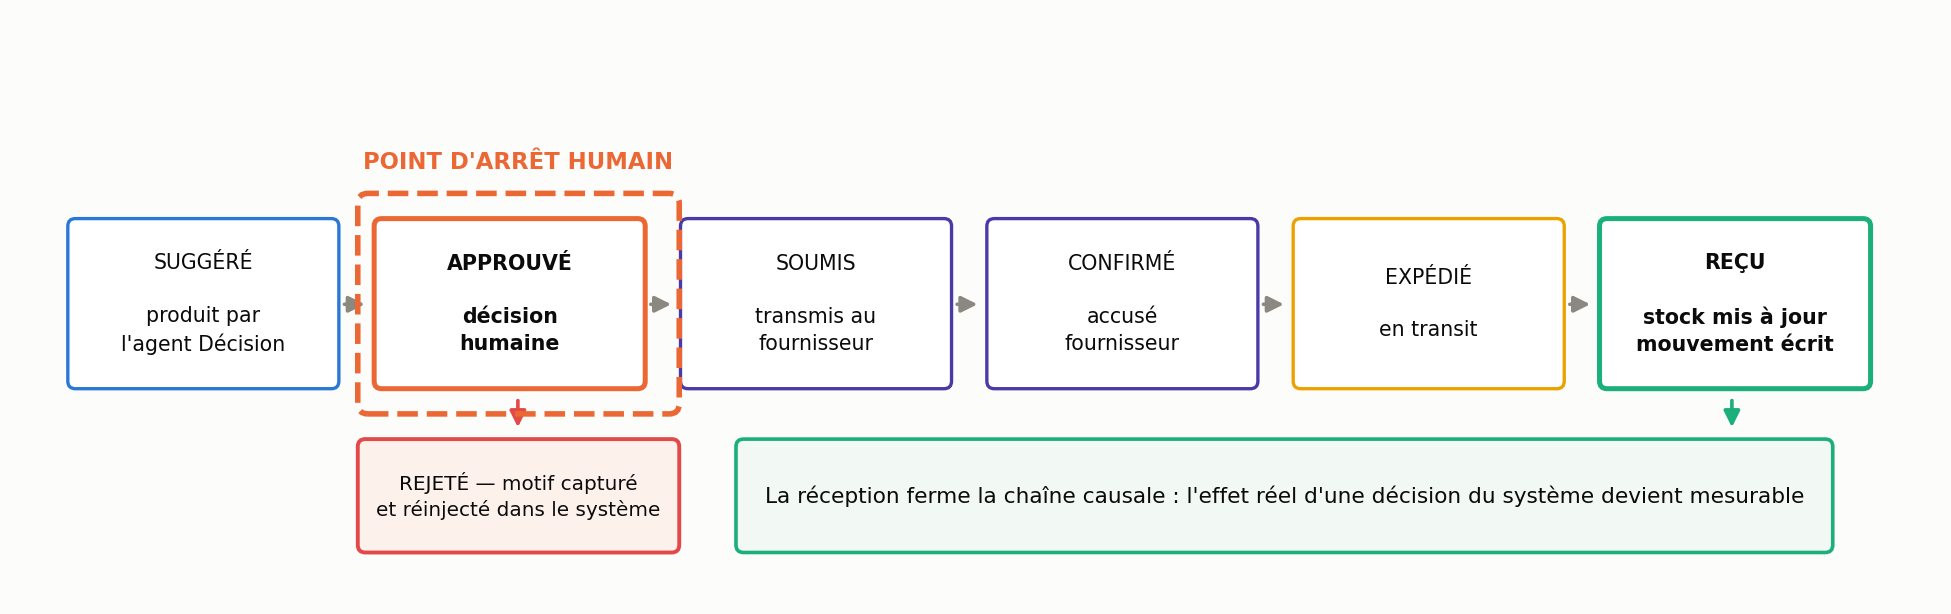
\includegraphics[width=\textwidth]{img/fig_cycle_bon_commande.png}
    \caption{Cycle de vie du bon de commande, de la suggestion à la réception}
    \label{fig:cycle-po-chap4}
\end{figure}

Une commande naît à l'état de \textbf{suggestion}, produite par l'agent Décision et rattachée à la recommandation qui la motive. Le responsable l'approuve, la modifie ou la rejette. Une fois approuvée, elle est transmise au fournisseur, suivie, puis réceptionnée totalement ou partiellement. La réception met à jour le stock et écrit le mouvement correspondant -- correction apportée à l'issue du chapitre~\ref{chap:donnees}. C'est cette écriture qui ferme la chaîne causale et rend mesurable l'effet réel d'une décision du système.

% ------------------------------------------------------------
\section{Robustesse de la chaîne de génération}
\label{sec:robustesse}
% ------------------------------------------------------------

Les agents génératifs dépendent de services externes, soumis à des indisponibilités, des limitations de débit et des variations de latence. L'exigence non fonctionnelle de robustesse impose que ces aléas ne se traduisent jamais par une absence de réponse. La figure~\ref{fig:cascade-chap4} présente la cascade retenue.

\begin{figure}[H]
    \centering
    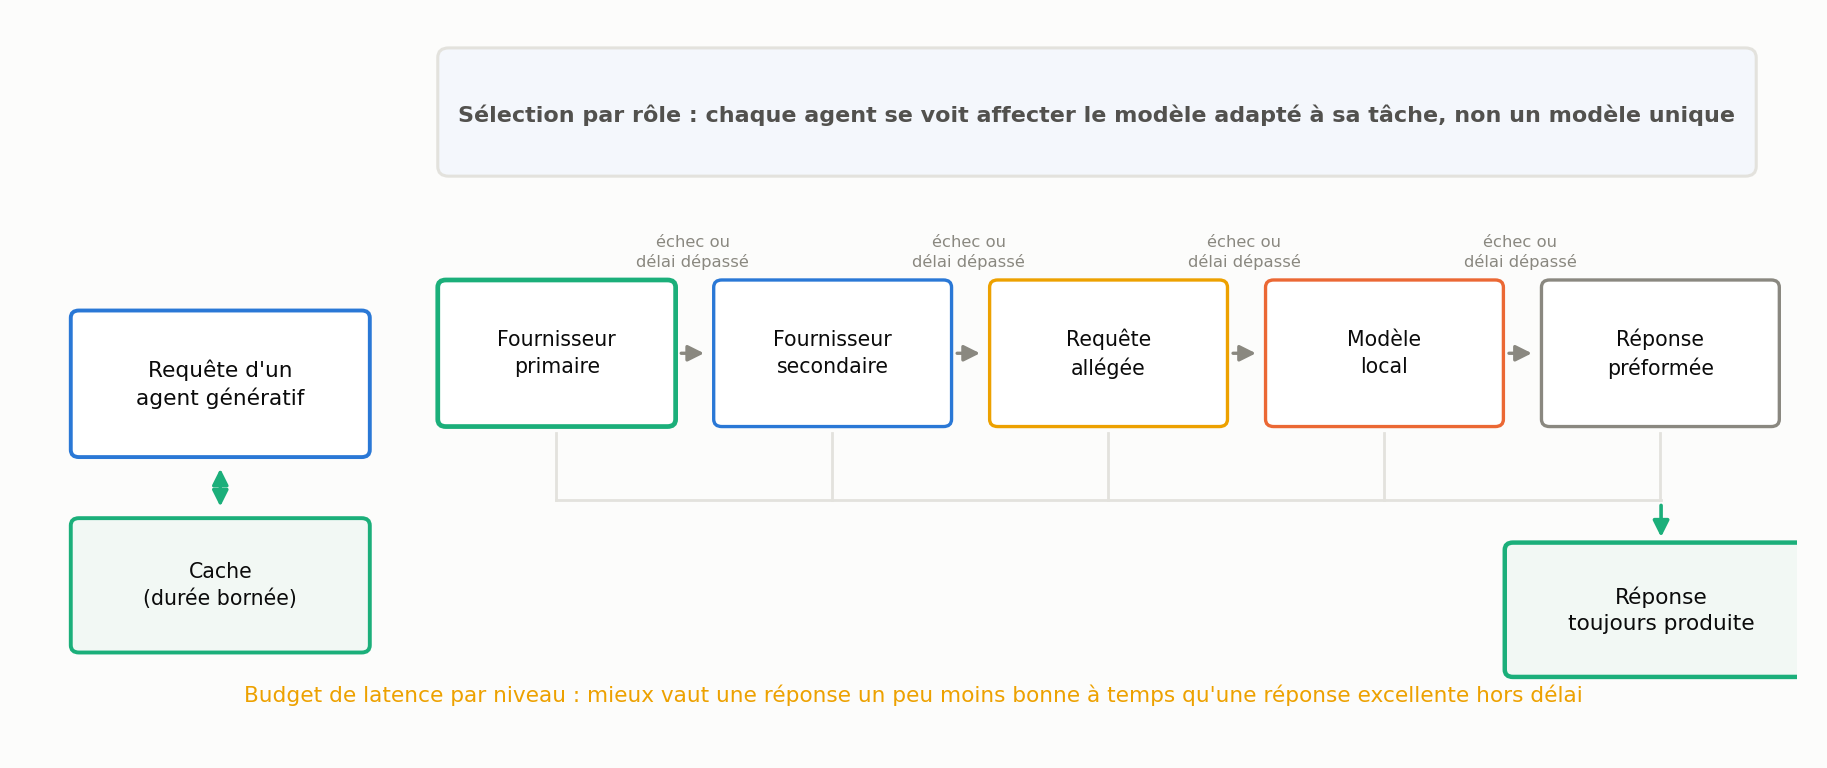
\includegraphics[width=\textwidth]{img/fig_cascade_llm.png}
    \caption{Cascade de repli de la chaîne de génération}
    \label{fig:cascade-chap4}
\end{figure}

Le mécanisme repose sur trois principes. La \textbf{sélection par rôle} affecte à chaque agent le modèle le mieux adapté à sa tâche, plutôt qu'un modèle unique : la génération d'une réponse conversationnelle et l'évaluation d'une recommandation n'ont ni les mêmes exigences de qualité ni les mêmes contraintes de latence. Le \textbf{repli en cascade} bascule vers un fournisseur alternatif en cas d'échec, puis vers une variante allégée de la requête, puis vers un modèle local, et enfin vers une réponse préformée dépendant de l'intention détectée. La \textbf{mise en cache} conserve les productions coûteuses et faiblement variables, notamment le contexte stratégique, pendant une durée bornée.

Un budget de latence est associé à chaque appel. Lorsqu'il est dépassé, la chaîne n'attend pas : elle bascule au niveau suivant de la cascade. Ce comportement traduit un arbitrage assumé -- une réponse un peu moins bonne immédiatement vaut mieux qu'une réponse excellente hors délai, dans un contexte où l'utilisateur est en situation de vente.

Le choix du modèle affecté à chaque rôle a été arrêté au terme d'une évaluation comparative dont les résultats sont présentés au chapitre~\ref{chap:evaluation}. Conformément à la règle de séparation entre annonce et mesure tenue dans ce rapport, aucun chiffre n'est avancé ici.

% ------------------------------------------------------------
\section*{Conclusion}
\addcontentsline{toc}{section}{Conclusion}
% ------------------------------------------------------------

Ce chapitre a conduit la quatrième phase de CRISP-DM. La sélection des techniques a été menée objectif par objectif, en confrontant les hypothèses de chaque technique candidate aux propriétés observées au chapitre~\ref{chap:donnees}, et en documentant les rejets autant que les choix. Le protocole de test a été conçu avant toute construction de modèle, avec des métriques justifiées et une comparaison systématique à une référence naïve.

Les modèles construits couvrent les huit objectifs analytiques. Le domaine Ventes repose sur un moteur de séries temporelles déterministe, complété d'un modèle appris global et organisé en cascade de repli. Le domaine Stocks superpose une base saisonnière et une correction contextuelle bornée, puis alimente des modèles de décision entièrement déterministes : stock de sécurité tenant compte de la double variabilité, point de commande, quantité économique ajustée aux contraintes fournisseurs, classification du risque à deux couches, arbre de décision à quatre branches dont une branche explicite de délégation à l'humain.

L'architecture agentique a été conçue autour d'un état partagé unique, dont la discipline d'écriture -- deltas seuls, fonctions de fusion, propriété exclusive des champs -- est ce qui rend le parallélisme possible. Le contrôle de conformité applique sept règles déterministes et route vers quatre issues, dont deux impliquent un humain. La chaîne de génération est protégée par une cascade de repli à plusieurs niveaux et un budget de latence.

Le principe énoncé en introduction a été tenu de bout en bout : sur les neuf unités du système, cinq n'invoquent aucun modèle de langage, et aucune valeur engageant une décision -- quantité, seuil, score, verdict -- n'est produite par génération. C'est cette propriété qui rend le système auditable, et donc validable par un responsable.

\textbf{Décision de fin de phase.} Les modèles sont construits, instrumentés et conformes au protocole de test conçu en section~\ref{sec:protocole-test}. Les techniques retenues en concurrence pour les objectifs OD-1 et OD-3 n'ont pas encore été départagées : ce départage relève de l'évaluation et non de la modélisation. La phase d'évaluation est autorisée ; elle fait l'objet du chapitre suivant.
